\documentclass[english,brazilian]{UNISINOSmonografia}
\usepackage[utf8]{inputenc} % charset do texto (utf8, latin1, etc.)
\usepackage[T1]{fontenc} 	% encoding da fonte (afeta a sep. de sílabas)
\usepackage{graphicx} 		% comandos para gráficos e inclusão de figuras
\usepackage{bibentry} 		% para inserir refs. bib. no meio do texto
\usepackage{placeins}		% manter imagens e tabelas no lugar especificado
\usepackage{enumitem}
\usepackage{xcolor}			% texto colorido no PDF
\usepackage{tabularx}		% permite especificar o tamanho das colunas de uma tabela

\usepackage{adjustbox}

\unisinosbst

%=======================================================================
% Dados gerais sobre o trabalho.
%=======================================================================
\autor{Gräbin}{Paulo Henrique Grolli}
\titulo{Insight: Um modelo acessível para localização em ambientes internos usando Bluetooth Low Energy}
\orientador[Prof.~Dr.]{Costa}{Cristiano André da}
\local{São Leopoldo}
\ano{2015}

%% dados específicos para monografia de Graduação
\unidade{Unidade Acadêmica Graduação}
\curso{Curso de Bacharelado em Ciência da Computação}
\natureza{%
Trabalho de Conclusão de Curso apresentado como requisito parcial
para a obtenção do título de Bacharel em Ciência da Computação
pela Universidade do Vale do Rio dos Sinos --- UNISINOS
}

% cada palavra-chave deve ser fornecida duas vezes, uma em português e
% outra no idioma estrangeiro (na verdade, em tantos idiomas quantos se
% desejar).
\palavrachave{brazilian}{Acessibilidade Ubíqua}
\palavrachave{brazilian}{Deficiência Visual}
\palavrachave{brazilian}{Sistemas de Posicionamento Indoor}
\palavrachave{english}{Ubiquitous Accessibility}
\palavrachave{english}{Visual Impairment}
\palavrachave{english}{Indoor Positioning System}

%=======================================================================
% Início do documento.
%=======================================================================
\begin{document}
\capa
\folhaderosto

%=======================================================================
% Dedicatória (opcional).
%=======================================================================
\begin{dedicatoria}
À meus pais que sempre me incentivaram na busca por conhecimento \\e a lutar pelos meus objetivos.\\[4ex] % quebra a linha dando um espaçamento maior

\begin{itshape} % faz o texto ficar em itálico
Learning is the only thing the mind never exhausts, \\
never fears, \\
and never regrets.\\
\end{itshape}
--- \textsc{Leonardo Da Vinci} % \textsc é o "small caps"
\end{dedicatoria}

%=======================================================================
% Agradecimentos (opcional).
%=======================================================================
\begin{agradecimentos}
Agradeço primeiramente ao meu orientador Cristiano André da Costa, pessoa a quem eu muito admiro, por ter me aceito como seu orientando, pelas valiosas conversas, seu auxilio incomparável e por sua disponibilidade sempre que necessário.

Aos meus pais, Ivani Grolli Gräbin e Milton Gräbin, que sempre me incentivaram a estudar e a realizar meus sonhos.

A minha namorada Victoria Caroline da Silva, pelas revisões, pela compreensão e por ficar sempre do meu lado.

Por último mas não menos importante, aos meus amigos, os quais não diretamente ajudaram na produção desse trabalho, mas são fundamentais e estiveram do meu lado nos momentos em que necessitava esvaziar a cabeça e entendiam os convites recusados.

Muito obrigado!

\end{agradecimentos}

%=======================================================================
% Epígrafe (opcional).
%
% ``[...] o autor apresenta uma citação, seguida de indicação de autoria,
% relacionada com a matéria tratada no corpo do trabalho. Podem, também,
% constar epígrafes nas folhas de aberturas das seções primárias.''
%=======================================================================
% \begin{epigrafe}
% ``\textit{Ninguém abre um livro sem que aprenda alguma coisa}''.\\
% (Anônimo)
% \end{epigrafe}

%=======================================================================
% Resumo em Português.
%=======================================================================
\begin{abstract}
Este trabalho apresenta a modelagem de um sistema de posicionamento em ambientes internos, com recursos de acessibilidade, desenhado com o objetivo de ser usado por pessoas com deficiência visual. O modelo consiste em uma aplicação a ser usada em dispositivos móveis, utilizando beacons transmissores Bluetooth espalhados pelo ambiente para obter a localização do usuário. O sistema objetiva fornecer uma localização confiável e um deslocamento seguro através de instruções de voz, leitura de tela e feedback tátil, para permitir que seus usuários possam se deslocar em ambientes desconhecidos sem a necessidade de auxílio de outras pessoas.
\end{abstract}

%=======================================================================
% Resumo em língua estrangeira
%=======================================================================
\begin{otherlanguage}{english}
\begin{abstract}
This paper presents the modeling of a Indoor Positioning System with accessibility features, designed used by visually impaired users. The model consists of an application used in mobile devices, making use of Bluetooth beacons deployed in the environment to obtain users location. The system aims to provide a reliable location and a safe and independent navigation using voice guidance, screen reading and haptic feedback in order to allow the users to navigate in unknown environments without need of assistance of other people.
\end{abstract}
\end{otherlanguage}

%=======================================================================
% Lista de Figuras (opcional).
%=======================================================================
\listoffigures

%=======================================================================
% Lista de Tabelas (opcional).
%=======================================================================
\listoftables

%=======================================================================
% Lista de Abreviaturas (opcional).
% Deve ser passada como parâmetro a maior das abreviaturas utilizadas.
%=======================================================================
% \begin{listadeabreviaturas}{seg., segs.}
% \item[ampl.] ampliado, -a
% \item[atual.] atualizado, -a
% \item[coord.] coordenador
% \item[N.~T.] Novo Testamento
% \item[seg., segs.] seguinte, -s
% \end{listadeabreviaturas}

%=======================================================================
% Lista de Siglas (opcional).
% Deve ser passada como parâmetro a maior das siglas utilizadas.
%=======================================================================
%\item[API] Application Programming Interface
%\item[SDK] Software Development Kid
%\item[UML] Unified Modeling Language
%\item[XML] Extensible Markup Language
\begin{listadesiglas}{SNPDPD}
\item[BLE] Bluetooth Low Energy
\item[GCM] Google Cloud Messasing
\item[GPS] Global Positioning System
\item[IBGE] Instituto Brasileiro de Geografia e Estatística
\item[IEEE] Institute of Electrical and Electronics Engineers
\item[JSON] Javascript Object Notation
\item[NFC] Near Field Communication
\item[PDV] Pessoas com Deficiência Visual
\item[REST] Representational State Transfer
\item[RFID] Radio Frequency Identification
\item[RLSB]	Royal London Society for Blind People
\item[SNPDPD] Secretaria Nacional de Promoção dos Direitos da Pessoa com Deficiência
\item[TAM] Technology Acceptance Model
\item[TTS] Text to Speech
\item[W3C] World Wide Web Consortium
\end{listadesiglas}

%=======================================================================
% Sumário
%=======================================================================
\tableofcontents

%=======================================================================
% Introdução
%=======================================================================
\chapter{Introdução} %Texto contextualizando o problema abordado e o escopo abarcado.

\epigrafecap{Now this is not the end. It is not even the beginning of the end.\\ But it is, perhaps, the end of the beginning}{Winston Churchill}

Pessoas com a visão saudável se apoiam enormemente no sentido da visão para se localizar. Frequentemente a sinalização destinada a orientação em locais como aeroportos, shopping centers e universidades é composta inteiramente por sinais visuais. Por esse mesmo motivo, pessoas com deficiência visual (PDV) têm grande dificuldade quando precisam deslocar-se, necessitando do auxílio de ferramentas como bengalas e cães-guia ou ainda da ajuda de outras pessoas. \citetexto{Ganz2014} afirma que a visão é o recurso mais importante na percepção do que se passa no entorno de alguém, e a sua perda significa uma severa redução na orientação e mobilidade, especialmente em ambientes desconhecidos e complexos.

O presente trabalho trata de uma alternativa para facilitar as atividades diárias das pessoas com deficiência, especialmente a visual, atuando na forma com que elas se orientam e se deslocam em ambientes internos. Será mostrada como alternativa a modelagem de um sistema que faz uso de conceitos como dispositivos móveis, acessibilidade ubíqua, tecnologias assistivas e localização por Bluetooth Low Energy (BLE).

Como resultado do trabalho, espera-se oferecer um sistema de fácil utilização que proporcione orientação e navegação precisas a seus usuários, de maneira que eles tenham confiança e independência. 

	\section{Motivação}
%Texto descrevendo a motivação para o trabalho, destacando a oportunidade de pesquisa encontrada e a motivação científica. Nessa seção cabe uma figura mostrando o problema atual e como será resolvido pelo trabalho sendo realizado.

% Na introdução você deve contextualizar o problema e mostrar por que vale a pena resolvê-lo. Você deve apresentar a solução proposta e mostrar o seu diferencial em relação aos trabalhos relacionados. Observe, porém, que na introdução você deve apenas tratar do O QUÊ e PORQUÊ, sem tratar do como \cite{Hexsel11}, que deve ser explicado na seção que descreve o trabalho desenvolvido.

De acordo com o levantado por \citetexto{IBGE2010}, no último Censo Demográfico, realizado em 2010, o Brasil possuía 45,6 milhões de pessoas que afirmaram ser portadoras de deficiência. Desse total, 35,7 milhões, ou 78,2\%, são pessoas com deficiência visual (PDV). Ou seja, aproximadamente 18\% da população brasileira é afetada.

A mesma pesquisa leva em consideração as diferentes intensidades da deficiência visual, aplicando os seguintes critérios \cite{IBGE2010}: 

\begin{quote}
	Foi pesquisado se a pessoa tinha dificuldade permanente de enxergar (avaliada com o uso de óculos ou lentes de contato, no caso de a pessoa utilizá-los), aplicando os seguintes critérios:
		
	• Não consegue de modo algum - para a pessoa que declarou ser permanentemente incapaz de enxergar; \\
	• Grande dificuldade - para a pessoa que declarou ter grande dificuldade permanente de enxergar, ainda que usando óculos ou lentes de contato; \\
	• Alguma dificuldade - para a pessoa que declarou ter alguma dificuldade permanente de enxergar, ainda que usando óculos ou lentes de contato; ou \\
	• Nenhuma dificuldade - para a pessoa que declarou não ter qualquer dificuldade permanente de enxergar, ainda que precisando usar óculos ou lentes de contato.
\end{quote}

Tendo diversas possíveis causas e atingindo pessoas em qualquer idade, a deficiência visual impõe severas dificuldades em todos os aspectos da vida dos que são afetados por ela. Educação, trabalho e vida social são exemplos, apenas para citar alguns. É difícil para uma pessoa com a visão perfeita se colocar no lugar de uma pessoa que não enxerga. \citetexto{quinones2011supporting} afirma que mobilidade e deslocamento são atividades naturais para aqueles que enxergam sem dificuldades, podendo ir e vir com relativa facilidade, já que pistas e sinais apontam a direção certa caso se percam, se vejam em situações desconfortáveis ou caso algum obstáculo apareça. Mostrando o outro lado, em \citetexto{URNA2007} são citadas algumas situações usuais que são impraticáveis para PDV, como, por exemplo, ler as linhas de ônibus que passam por uma determinada parada ou ainda ler o destino de um ônibus se aproximando. Conforme \citetexto{rodriguez2014accessible}, PDV não possuem a totalidade da informação de que necessitam para contornar obstáculos. O mesmo se aplica a direção seguida e a distância remanescente até o destino, informações essenciais para um deslocamento em qualquer ambiente. Não poder ver a sinalização na rua ou semáforos em um cruzamento torna perigoso para PDV transitarem desacompanhados, necessitando ter a companhia de amigos ou familiares durante todo o trajeto. 
Em \citetexto{Ganz2014}, os autores afirmam que, mesmo com auxílio de um cão-guia ou bengala, ainda é um desafio enorme para os PDV se deslocarem em tais ambientes sem ajuda de uma pessoa com visão plena. 
\citetexto{dias2015navpal} afirma que é esperado que PDV explorem ambientes internos por conta própria, ou então levem consigo seus próprios acompanhantes ou ferramentas. Existem estabelecimentos, como, por exemplo, o metrô de Porto Alegre, que coloca uma parte de seus funcionários à disposição dos deficientes para guiá-los durante seu trajeto. Porém, seu número é limitado, o que faz com que os usuários precisem esperar até um funcionário estar disponível. Além disso, muitas vezes essas pessoas não receberam treinamento sobre como acompanhar corretamente um deficiente visual.

Em 2014, a Royal London Society for Blind People (RLSB), organização sem fins lucrativos que busca criar uma diferença que melhore a vida das futuras gerações de PDV, divulgou um manifesto para chamar atenção aos desafios enfrentados diariamente pelos PDV, que os impedem de usufruir da totalidade dos seus direitos fundamentais. \cite{YouthManifesto}. Desafios esses que não são restritos às divisas do Reino Unido, onde a organização se encontra.
De acordo com o documento, perda de visão é uma experiência tão traumática que pode ser comparada à perda de um ente querido, visto que dificilmente eles recebem o apoio emocional necessário. Não conseguir enxergar causa isolamento social, o que prejudica enormemente o futuro do indivíduo. Ainda é dito que empresas ou organizações, como lojas, bancos e agentes de viagem, não compreendem as necessidades e habilidades dos PDV, impedindo-os de levar uma vida comum e impossibilitando-os de realizar as atividades que gostariam. O trabalho ainda destaca que, frequentemente, as pessoas não sabem oferecer assistência básica, como guiá-los em espaços públicos, estações de trem, por exemplo. Dentre as áreas citadas como problemáticas, é possível destacar a mobilidade urbana, a educação superior e acessibilidade na tecnologia. No trabalho ainda é revelado o motivo de sua publicação, informando que 25\% das pessoas com perda de visão estão insatisfeitas com suas vidas. \cite{YouthManifesto}.

Em relação à mobilidade, \citetexto{YouthManifesto} cita que existe uma variedade de aplicativos para smartphone que auxiliam pessoas a se localizar e se deslocar, porém, poucos deles são acessíveis. É afirmado também que, se essas tecnologias fossem projetadas com todas as pessoas em mente, mais PDV poderiam transitar com segurança, reduzindo a dependência de outras pessoas. 

Indo ao encontro das iniciativas das RLSB e atuando na área de mobilidade, o modelo proposto visa auxiliar portadores de deficiência visual a se localizar e se deslocar em ambientes internos, como, por exemplo, o campus de uma universidade, buscando facilitar o acesso à educação e à vida social disponível nos campi. Usando dispositivos móveis, o sistema irá informar ao usuário sua localização atual e recomendar caminhos que o levem ao seu destino, levando em consideração os obstáculos em sua rota.

Tendo a premissa de funcionar a partir do smartphone do usuário, o sistema será projetado para ter usabilidade intuitiva e ser uma parte quase invisível do cotidiano do usuário, aplicando o conceito de computação ubíqua introduzido em \citetexto{Weiser1991}, a fim de se adaptar às necessidades dos PDV.

	\section{Questão de pesquisa}
	Tendo identificado e contextualizado o problema, foi definida a seguinte questão de pesquisa a ser explorada neste trabalho:

	Como a Computação Ubíqua pode contribuir no desenvolvimento de um modelo de sistema que seja uma alternativa ao problema de localização e deslocamento em ambientes internos enfrentado por deficientes visuais, promovendo acessibilidade e permitindo o trânsito com confiança e independência?

	A questão de pesquisa atua como o norteador do trabalho: após tê-la definido, é buscada a criação de um modelo que contemple todos os aspectos dela. Em outras palavras, uma vez proposta a questão, o trabalho irá respondê-la através do modelo proposto.

	Neste trabalho serão usados conceitos como sensibilidade ao contexto, computação móvel e uso de sensores. Conceitos esses que surgem após a definição de computação ubíqua. Através da aplicação desses conceitos, o objetivo do trabalho é conceber um modelo de software acessível, no sentido de ser mais uma ferramenta assistiva, capaz de auxiliar seus usuários em momentos em que eles precisam saber sua localização e se deslocar em ambientes internos, como, por exemplo, o campus de uma universidade. O modelo emprega métodos alternativos para se comunicar com o usuário, não se limitando ao texto puro, mas usando também voz e vibração.

	\section{Objetivos}
	Tendo identificado a questão de pesquisa, foram definidos alguns objetivos para este trabalho, apresentados nas seções subsequentes.
	
		O objetivo principal é especificar, desenvolver e validar um modelo de sistema para localização e orientação de PDV em ambientes internos através de dispositivos móveis, aplicando fundamentos de acessibilidade e conceitos de computação ubíqua, para permitir que seus usuários se localizem e se desloquem em ambientes desconhecidos sem necessidade do auxílio de outras pessoas.

		O sistema não deve exigir uso de hardware dedicado por parte dos usuários, devendo, porém, ser leve, discreto, preciso e de fácil uso. \\
		
		Para atingir o objetivo geral deste trabalho, foram definidos os seguintes objetivos específicos:

		\begin{itemize}
			\item Compreender as limitações impostas pela deficiência visual - estudar essa deficiência buscando entender a maneira com que ela altera a vida de seus portadores e como afeta suas capacidades, bem como entender as necessidades que surgem a partir dela, de forma a contribuir para o seu bem-estar.

			\item Compreender computação móvel e ubíqua - analisar quais características da computação móvel e ubíqua são desejáveis em um modelo que será usado por PDV, de forma que o modelo se integre ao cotidiano de seus usuários da maneira mais natural e intuitiva possível.

			\item Compreender sistemas de localização e navegação - analisar trabalhos e soluções existentes nessa área, buscando entender quais características deles podem ser aproveitadas em um sistema para PDV, bem como novas características que devem ser incorporadas para que as necessidades dos PDV sejam atendidas.

			\item Desenvolver um protótipo da solução - modelar e codificar uma parte do modelo proposto, criando um protótipo que utilize o conhecimento adquirido e possibilite a avaliação do modelo.

			\item Avaliar o sistema desenvolvido - testar o sistema em campo e avaliar, fazendo uso de questionário, a eficácia e eficiência do sistema. O resultado ajudará identificar a aceitação, pontos fortes e possíveis melhorias do sistema, bem como elencar trabalhos futuros relacionados ao tema.
		\end{itemize}

	\section{Organização do texto}
O presente trabalho está dividido em seis capítulos. 
O segundo capítulo apresenta os principais conceitos utilizados para o embasamento desde trabalho, descrevendo computação móvel e ubíqua, tecnologias assistivas, sistemas de localização e dando um panorama geral sobre a deficiência visual.
O terceiro capítulo apresenta os trabalhos relacionados feitos nesta área, cobrindo seus aspectos mais relevantes e traçando um comparativo entre eles.
No quarto capítulo é feito um detalhamento do modelo proposto neste trabalho, dando ênfase na arquitetura do sistema, seus principais requisitos e componentes que formam este modelo.
O quinto capítulo descreve a metodologia de pesquisa aplicada no trabalho, materiais utilizados e como será realizado o desenvolvimento do protótipo.
O sexto e último capítulo conclui o trabalho e apresenta as considerações finais, uma comparação com os trabalhos relacionados e sugestões de trabalhos futuros.

% %=======================================================================
% % Fundamentação teórica
% %=======================================================================
\chapter{Fundamentação Teórica}
\epigrafecap{The obvious is that which is never seen until someone expresses it simply}{Khalil Gibran}
% Esse capítulo contém os principais conceitos e áreas envolvidos no trabalho. O capítulo deve apresentar esses conceitos em uma linha de pensamento sequencial e encadeada. Não deve conter subseções independentes sem se relacionar uma com a outra. O capítulo inicia explicando sua lógica e todas as subseções são ligadas entre si por uma sequência lógica de pensamento e redação.
Este capítulo apresenta a base teórica sobre a qual está construído este trabalho. Inicialmente é apresentada uma visão geral sobre computação ubíqua, computação móvel e acessibilidade. Em seguida os conceitos são mesclados, e então é introduzido o conceito de acessibilidade ubíqua e tecnologias assistivas. Finalmente, é introduzida a tecnologia Bluetooth, seu modo de funcionamento e aplicações práticas.

	\section{Computação Móvel e Ubíqua}
Tecnologias tão avançadas que deixam de ser um fim em si mesmas e passam a ser um meio para que as pessoas realizem seus afazeres. Tão conectados, tão presentes em nossa rotina e concebidas para naturalmente se integrarem em nossas vidas que deixam de ser notadas e se colocam no plano de fundo da nossa percepção. É assim que \citetexto{Weiser1991} começa introduzindo o conceito de computação ubíqua. O autor também a conceitua como "uma nova maneira de pensar a respeito de computadores no mundo". \cite{Weiser1991}.

Weiser previu um mundo onde computadores deixariam de possuir apenas o tamanho de um notebook que é usado em cima de uma mesa. Um mundo onde computadores seriam pequenos o suficiente para serem embutidos em botões de uma camisa e também grandes o suficiente para ocuparem os ambientes em que convivemos, estudamos ou trabalhamos. Esses computadores conversariam entre si de maneira contínua e transparente, de modo que eles e todos os usuários estariam permanentemente conectados, permitindo que serviços estejam acessíveis em todos os lugares e em todos os momentos. Tal definição vai ao encontro do conceito estabelecido por \citetexto{Satyanarayanan2001} para computação móvel como sendo: “Informação na ponta dos dedos, em qualquer lugar e em qualquer tempo”.

A computação ubíqua, em outras palavras, consiste em trazer e integrar a computação ao mundo real. Conforme \citetexto{ballance2008developing}, é um conceito diametralmente oposto a ideia de realidade virtual. O autor ainda afirma que a computação ubíqua oferece potencial para diminuir ou ainda eliminar as intervenções humanas necessárias em qualquer sistema computacional.

Essa área de pesquisa ainda traz consigo conceitos fundamentais para uma devida compreensão do termo. A heterogeneidade da rede é garantida por padrões que possibilitam que dispositivos criados por diferentes fabricantes, para diferentes finalidades, com diferentes softwares e hardwares, se conectem através da internet. A integração com o mundo real possibilita a inserção de computadores e sensores em diversos artigos comuns do dia-a-dia, gerando informações sobre costumes e preferências dos usuários que permitem uma nova geração de serviços inteligentes e cuidadosamente personalizados. Computação na nuvem, sistemas distribuídos, computação móvel e internet são termos que andam de mãos dadas e servem como base para garantir que os conceitos anteriormente apresentados estejam sempre disponíveis e ao alcance dos dedos em segundos em qualquer lugar do mundo.

Um dos aspectos mais interessantes da computação ubíqua é a ciência de contexto, definida em \citetexto{dey2001understanding} como o uso de informações relevantes, tais como localização, preferência, histórico e horário podem ser usadas para determinar a situação em que o usuário se encontra. Tais informações servem para que os softwares desenvolvidos possam se adaptar as necessidades e reagir, instantânea e transparentemente, às mudanças no ambiente em que o usuário se encontra.

Com a computação cada vez mais onipresente, juntamente com dispositivos móveis e poderosos, é possível aplica-la na tentativa de melhorar a vida das pessoas. Uma das possíveis aplicações é na promoção da acessibilidade de quem necessita.

	\section{Acessibilidade}
Acessibilidade representa o direito de acessar informações; eliminação de barreiras arquitetônicas; de disponibilização de comunicação; de acesso físico; de equipamentos e programas adequados; de conteúdo e apresentação da informação em formatos alternativos – não se restringindo somente a internet –, a fim de melhorar a qualidade de vida de pessoas com algum tipo de deficiência. \cite{AcessibilidadeBrasil}. 

% Legislação
No Brasil existe legislação específica para assegurar os direitos individuais de todos os cidadãos. Como exemplo podem ser citadas a lei 5.296/2004, conhecida como lei da acessibilidade, e as leis 10.048/00 e 10.098/00. Juntas, estabelecem normas e critérios básicos para a promoção da acessibilidade, descrevendo regras de construção de espaços públicos, edifícios de uso público e privado. Elas ainda regulamentam como deve se dar a acessibilidade nos sistemas públicos de comunicação e sinalização e normas para promoção da acessibilidade. Também podem ser citados os Decretos 3.298/99 e 5.296/04, que caracterizam o que é deficiência, bem como o que é necessário para que alguém seja considerado pessoa portadora de deficiência física. No aspecto tangível, a legislação brasileira é eficaz ao garantir direitos dos PDV.

% Acessibilidade na tecnologia
Entretanto, a vida digital foge da alçada da jurisdição de qualquer país. Em busca de tornar a internet um lugar mais acessível para todas as pessoas, entram em cena organizações como o Institute of Electrical and Electronics Engineers (IEEE) e o World Wide Web Consortium (W3C), que publicam orientações e diretrizes numa tentativa de garantir acessibilidade universal da web. Nenhuma empresa ou desenvolvedor é formalmente obrigado a aplicar essas diretrizes em seus sites e produtos, todavia, o fazem com o objetivo de atrair mais clientes ou visitantes. As recomendações não são direcionadas para uma tecnologia específica, podendo ser utilizadas em qualquer aplicação, linguagem ou navegador de internet. \cite{W3Cguideliness}. Segundo \citetexto{rodriguez2014accessible}, um aspecto que deve ser considerado é que a aplicação seja acessível para um grande número de pessoas, independentemente das necessidades dos usuários, devendo-se usar diversos canais sensoriais (visual, auditivo e tátil) para passar as informações. Porém, é importante ressaltar que a acessibilidade da web não é baseada apenas na acessibilidade do conteúdo disponibilizado, e sim nos diversos agentes e componentes, como navegadores, usuários, desenvolvedores e ferramentas de desenvolvimento, trabalhando juntos para oferecer uma melhor experiência ao usuário.

De acordo com \citetexto{vanderheiden2008ubiquitous}, no início dos anos 90 apenas computadores fabricados pela Apple contavam com recursos de acessibilidade, enquanto nos demais, softwares de terceiros eram a alternativa para aqueles que necessitavam. Graças aos esforços combinados da indústria e da academia, hoje todos os maiores sistemas operacionais possuem recursos de acessibilidade, como leitores de tela e lente de aumento, nativos entre suas funcionalidades. Pensados e concebidos diretamente na construção do sistema operacional, esses recursos são capazes de oferecer uma integração mais profunda com o sistema e uma experiência muito melhor ao usuário se comparados a softwares produzidos por outras empresas. 

Em consonância com a afirmação de \citetexto{Weiser1991}, \citetexto{vanderheiden2008ubiquitous} diz que, com a computação substituindo o paradigma de computação pessoal para computação ubíqua, é necessário pensar em novas formas de acessibilidade:

\begin{quote}
	Algum dia computadores serão como as lâmpadas de hoje. Houve uma época em que tínhamos que carregar lâmpadas conosco a qualquer lugar que fossemos. As pessoas carregavam consigo lanternas ou velas pelos quartos ou a qualquer lugar onde quisessem ir. Não havia expectativa de que luz seria fornecida a menos que cada um trouxesse a sua. Hoje em dia, ninguém mais carrega lâmpadas. As pessoas esperam que, exceto quando acampando ou viajando pela floresta, diversas fontes de luz sejam oferecidas nos lugares onde elas entram. No futuro podemos esperar uma situação semelhante em relação à computação. Onde quer que se vá, a computação estará através de diversos tipos de interfaces. Talvez tenhamos que levar conosco tipos específicos de interfaces se assim desejarmos, mas seremos capazes de usá-las juntamente com os recursos dos ambientes em que estaremos. \cite{vanderheiden2008ubiquitous}
\end{quote}

Assim emergem os conceitos de acessibilidade ubíqua e interfaces de usuário plugáveis, como talvez a forma definitiva de acessibilidade. Esses conceitos são descritos por \citetexto{Tavares2011} como a capacidade de invocar recursos assistivos especiais diretamente da internet para serem usados em qualquer tela próxima.

\citetexto{Tavares2011} define a acessibilidade ubíqua, também chamada de u-accessibility, como a união entre as normas e padrões para acessibilidade; tecnologias e interfaces que atendem às necessidades dos usuários; e computação ubíqua, através de dispositivos móveis, sensores e a comunicação entre eles.

	\section{Tecnologias Assistivas}
\citetexto{pupo2006acessibilidade} afirma que existem tecnologias assistivas para auxiliar no acesso às informações, na comunicação, durante a locomoção e em atividades comuns no dia-a-dia, como estudo, trabalho e lazer, citando como exemplos cadeiras de rodas, bengalas, próteses, lupas e aparelhos auditivos. Conforme \citetexto{dias2015navpal}, tecnologias assistivas desempenham um papel chave na independência e segurança de pessoas com deficiência. Para os PDV, tecnologias assistivas bem planejadas e bem implementadas podem fazer significante diferença na educação, aceitação social e produtividade. \cite{dias2015navpal}. Tecnologias assistivas são formas bastante eficazes de promoção de acessibilidade.

Não há um conceito universalmente estabelecido e aceito de tecnologias assistivas. Diversas entidades e países buscam estabelecer sua própria definição. O Brasil apresenta seu conceito em \cite{TA2009}, descrevendo-o como se segue:
\begin{quote}
	Tecnologia Assistiva é uma área do conhecimento, de característica interdisciplinar, que engloba produtos, recursos, metodologias, estratégias, práticas e serviços que objetivam promover a funcionalidade, relacionada à atividade e participação, de pessoas com deficiência, incapacidades ou mobilidade reduzida, visando sua autonomia, independência, qualidade de vida e inclusão social.
\end{quote}

Conforme \citetexto{stewart2008accessible}, é preferência dos usuários, tanto PDV como aqueles com visão saudável, carregar consigo dispositivos que caibam em um bolso, deixando as mãos livres. O autor ainda afirma que PDV consideram essencial que os aparelhos sejam imperceptíveis durante seu uso. No mesmo sentido, \citetexto{taylor2012smart} diz que PDV preferem não atrair atenção para si enquanto fazem uso de um sistema de localização.

Diversos autores destacam as vantagens do uso de smartphones como dispositivos capazes de oferecer acessibilidade em diversas formas aos usuários. Segundo \citetexto{Ganz2014}, smartphones, item básico possuído por grande parte da população, têm se mostrado uma ferramenta capaz de beneficiar enormemente os PDV em sua vida diária, através de aplicações, como leitores de cédulas de dinheiro, reconhecimento de cores e objetos, navegação na web, leitura de e-mails e ligações telefônicas. O trabalho ainda afirma que o uso de smartphones é possível devido à presença de recursos de acessibilidade oferecidos pelos principais sistemas operacionais disponíveis. Entre esses recursos, podemos destacar a leitura de telas e os alertas vibratórios, essenciais para aqueles que não enxergam as telas sensíveis ao toque que equipam a grande maioria dos smartphones disponíveis atualmente. Ao invés de apenas ler o texto sendo exibido, essa funcionalidade também informa sobre os tipos de cada componente, possibilitando ao usuário saber como interagir com cada um.

De acordo com \citetexto{Brady2013}, os maiores sistemas operacionais para dispositivos móveis disponíveis incluem por padrão a funcionalidade de leitura de tela, de maneira a permitir seu uso por usuários PDV. Aparelhos com tela sensível ao toque eram tidos como inacessíveis a usuários cegos, porém interfaces multitoque bem desenhadas aproveitam melhor o tamanho da tela e são preferidos pelos deficientes visuais.

\citetexto{mau2008blindaid} afirma que a utilização de um dispositivo de uso geral possui uma clara vantagem sobre um aparelho específico que os usuários teriam que carregar e aprender a usar. Os autores ainda definem o telefone celular como “a peça de tecnologia mais valiosa para os cegos”. \cite{mau2008blindaid}. Conforme \citetexto{URNA2007}, a comunidade PDV recebeu muito bem o uso de smartphones, e tem categorizado os aparelhos como um computador ideal para acessibilidade.

Segundo o estudo realizado por \citetexto{quinones2011supporting}, PDV possuem o desejo de carregar consigo a menor quantidade possível de equipamento. É necessário criar tecnologias que não sejam um fardo a ser carregado, mas que ofereçam a quantidade apropriada de informações ao usuário. Uma maneira citada pelo autor é a incorporação de tecnologias de navegação em aparelhos que deficientes visuais carreguem consigo normalmente, assim reduzindo o número de objetos que devem ser cuidados. Smartphones se encaixam perfeitamente nessas necessidades, revelando-se como dispositivo perfeito para ser usado no desenvolvimento de novas tecnologias que visam promover acessibilidade.

Em \citetexto{narasimhan2009smartphone} são sugeridos alguns princípios que devem ser seguidos no desenvolvimento de ferramentas assistivas para PDV:
\begin{itemize}
	\item A ferramenta deve possibilitar a independência nas atividades diárias, não exigindo a assistência e/ou acompanhamento de outras pessoas, com deficiência visual ou não.
	\item Evitar adicionar melhoramentos nas bengalas, visto que aumentar o peso ou novas funcionalidades podem influenciar negativamente no uso diário
	\item Usuários devem ter a opção de usar ou não usar as funcionalidades disponíveis. Seu uso não pode ser forçado para não dificultar seu dia-a-dia.
	\item Manter custos baixos é promover a adoção de produtos pra PDV, já que produtos específicos para esse público tendem a ser mais caros.
\end{itemize}

Baseando-se nestes princípios e na capacidade de auxílio dos smartphones, um exemplo de ferramenta assistiva que vem à tona é o uso de dispositivos móveis para que o usuário deficiente visual obtenha sua localização atual e, a partir dela, descubra locais e recursos acessíveis ao seu redor. Tal ferramenta exige a utilização de alguma tecnologia capaz de distinguir e obter a posição do usuário. Uma das tecnologias capazes de atender a essas necessidades é o Bluetooth.

	\section{Tecnologia Bluetooth}
Bluetooth é uma tecnologia de comunicação sem fios de curto alcance, lançada comercialmente em 1990, quando teve sua primeira especificação formal divulgada. Desde então, diversas modificações foram feitas e a tecnologia passou por diversos aprimoramentos, estando atualmente na versão 4, também conhecida como Bluetooth Smart ou Bluetooth Low Energy, lançada em 2010. A tecnologia nativamente possui capacidade para lidar com diversos serviços, tais como criptografia, transferência de arquivos e transferência síncrona e assíncrona de dados.

O Bluetooth foi criado e atualmente é mantido por um conjunto de empresas conhecido como Bluetooth Special Interest Group (SIG). Inicialmente formado por Ericsson, Intel, Nokia, Toshiba e IBM, o SIG é hoje composto por mais de 20.000 empresas, incluindo Apple, Microsoft, Motorola e Lenovo.

A tecnologia possui duas formas distintas de atuação, apesar de compartilharem entre si alguns pontos em comum. O primeiro e mais antigo modo, disponível desde a primeira especificação, é chamado Basic Rate (BR). O segundo foi introduzido somente na versão 4 e é chamado Low Energy (LE) e é o modo que será utilizado pelo modelo proposto neste trabalho.

De acordo com \citetexto{Townsend2014}, o LE foi criado para permitir produtos que requerem baixíssimo consumo de energia e baixo custo, quando comparados ao outro modo. Assim sendo, esse modo foi pensado para aplicações que exigem pouca troca de informações. Um exemplo de produto viável com a chegada do modo LE são os beacons Bluetooth, que consistem em dispositivos do tamanho de uma moeda comum, compostos por um processador, uma bateria e um transmissor, que transmitem informações sobre si em intervalos regulares. Como o sinal dos beacons tem seu alcance limitado a alguns poucos metros, foi introduzido o conceito de microlocalização, tornando possível o desenvolvimento de novas aplicações e serviços onde antes não era possível, tais como lojas, grandes shows ou eventos, estádios esportivos e em ambientes internos. A microlocalização é definida por \citetexto{zafari2015micro} como a obtenção da localização de uma entidade com grau de precisão na ordem dos centímetros. 

A imensa maioria dos telefones celulares hoje faz uso nativo da tecnologia, não exigindo qualquer tipo de equipamento adicional. Os sistemas operacionais Android e iOS oferecem suporte a tecnologia a partir das versões 4.3 e 5, respectivamente. Ao contrário da versão anterior, a partir da versão 4, a tecnologia Bluetooth não exige o pareamento de dispositivos para que eles possam se localizar e comunicar.

De acordo com \citetexto{ballance2008developing}, a combinação computação ubíqua e Bluetooth tem potencial para fomentar soluções simples e baratas que outrora não seriam possíveis.

\citetexto{taylor2012smart} revelam que diversas tecnologias foram utilizadas anteriormente em modelos de sistema para localização e navegação para PDV, tanto em ambientes internos como externos. Sonares, Radio Frequency Identification (RFID), Near Field Communication (NFC), Bluetooth e Global Positioning System (GPS) são algumas delas. Os autores ainda apontam que, apesar de todas elas oferecerem vantagens em suas propostas, todas também possuem pontos fracos:

\begin{itemize}
  \item GPS é normalmente usado para localização em ambientes externos, mas se mostra ineficiente devido à própria natureza das ondas de rádio usadas na tecnologia, quando obstáculos são locados ao redor do usuário. De acordo com \citetexto{montague2010accessible}, apesar de GPS ser muito eficiente na hora de determinar um ponto em um mapa, essa tecnologia está longe ser a melhor escolha para ambientes internos. Nesse cenário é preciso viabilizar a possibilidade de diversos andares em um local, o que não é possível ser feito via GPS.
  \item Sonares são formas baratas de detecção de objetos e obstáculos, através de frequências acústicas, mas exigem hardware dedicado e não servem para localização.
  \item RFID, juntamente com NFC, exige proximidade de seus emissores para que a comunicação seja estabelecida.
  \item Os autores não chegam a citar nominalmente os pontos fracos da tecnologia Bluetooth, mas um grande ponto que pode ser citado é o consumo de bateria causado pelas versões que antecederam a versão 4, também chamada de Bluetooth Low Energy.
\end{itemize}

A Tabela \ref{tab:tecnologiasLocalizacao} mostra algumas características dessas tecnologias.

\begin{table}
	\caption{Tabela comparativa entre tecnologias aplicadas em localização}
	\label{tab:tecnologiasLocalizacao}
		\begin{tabular}{ p{2,5cm} | p{2cm} | p{2,5cm} | p{3cm} | p{3cm} }
			\hline
				Tecnologia & Precisão & Abrangência & Suportada por smartphones & Exige linha de visão   \\ \hline
				GPS & 10 m & Externo & Praticamente todos & Não   \\ \hline
				Bluetooth 2 & 100 m & Ambos & Praticamente todos & Não   \\ \hline
				Bluetooth BE & 100 m & Ambos & Alguns & Não   \\ \hline
				RFID & Entre 10cm e 100m & Ambos & Alguns & Não   \\ \hline
				NFC & Até 10 cm & Ambos & Alguns & Não   \\ \hline
				Ultrassom & Centímetros & Ambos & Poucos & Não   \\ \hline
				Infravermelho & Centímetros & Ambos & Poucos & Sim   \\ \hline
			\end{tabular}
		\fonte{\citetexto{stewart2008accessible}}
\end{table}

Analisando a tabela podemos ver que a tecnologia GPS é a que oferece a maior precisão na localização, além de ser suportada pela maioria dos smartphones. Porém, ela não é recomendada para ambientes internos. As tecnologias ultrassom e infravermelho oferecem boa precisão, mas são pouquíssimos os modelos de smartphone que fazem uso delas. Infravermelho ainda exige contato visual direto e sem restrições entre os dispositivos para funcionar. RFID e NFC oferecem ótima precisão devido à proximidade necessária para uso da tecnologia, porém, possuem pouco suporte por parte dos dispositivos. Bluetooth, em ambas as versões, possuem precisão média e são bem suportadas pelos smartphones.

Importante ressaltar que os dados apresentados são limites teóricos da tecnologia obtidos através da especificação de cada uma das tecnologias. Estes valores podem variar para mais ou para menos, visto que, segundo \citetexto{Townsend2014}, o alcance de qualquer tecnologia sem fio é influenciado por diversos fatores, entre eles é possível  citar o ambiente onde ela está sendo utilizada, design da antena de transmissão o material utilizado.

%=======================================================================
% Trabalhos relacionados	
%=======================================================================
\chapter{Trabalhos Relacionados}\label{cap:trabalhosRelacionados}
\epigrafecap{The most dangerous phrase in the language is "We have always done this way"}{Grace Hopper}
% Essa atividade consiste em detalhar os trabalhos relacionados. O capítulo começa apresentando como os trabalhos relacionados foram escolhidos. A seguir, existe uma seção descrevendo cada trabalho relacionado. Por fim, uma seção compara os trabalhos relacionados, apresentando a tabela criada na atividade 2 e descrevendo as lacunas que serão abordadas pela presente dissertação.

Para criar um novo modelo em busca de mitigar um problema enfrentado pelas pessoas com deficiência visual, é necessário buscar outros trabalhos com foco na mesma área, a fim de identificar falhas e virtudes de cada um, gerando um comparativo entre eles. Foram encontrados diversos trabalhos que compartilham do objetivo deste através do emprego de propostas tecnológicas. Para a escolha daqueles que seriam apresentados neste capítulo foi feita uma seleção, levando em consideração critérios como a similaridade do objetivo com o deste trabalho, o ano de publicação do modelo, suporte à acessibilidade, foco em dispositivos móveis e a abrangência de ambientes internos. Dessa forma, os selecionados foram os trabalhos mais recentes que promovam acessibilidade, usem dispositivos móveis, atuem principalmente em ambientes internos e possuam objetivos mais semelhantes com o deste trabalho.

Neste capítulo, são apresentadas quatro soluções que possuem propósito semelhante, bem como características desejadas por esse trabalho. Ao final desde capítulo, no item~\ref{comparacaoTrabs}, é apresentado um comparativo entre os trabalhos selecionados, destacando pontos que são relevantes para o desenvolvimento da arquitetura do presente trabalho.

%=======================================================================
% PERCEPT
%=======================================================================
	\section{PERCEPT: Indoor Navigation for the Blind and Visually Impaired} 
\citetexto{Ganz2011} e \citetexto{Ganz2012} introduzem um sistema de sistema de localização que busca auxiliar PDV aumentando sua percepção dos ambientes internos. O sistema é composto por um servidor central, responsável por armazenar as informações de localização do ambiente, tags RFID passivas distribuídas pelo local, leitores RFID acoplados em luvas utilizadas pelos usuários em conjunto com um smartphone Android. O principal motivo que levou à escolha do RFID é a granularidade que a tecnologia permite graças ao baixo custo de implantação e ao fato de elas não exigirem fonte de alimentação elétrica. De acordo com os autores, a diferença do PERCEPT em relação a outros sistemas similares é a combinação luva/leitor e smartphone e também o baixo custo de implantação e manutenção. 

A arquitetura do sistema também é descrita em \citetexto{Ganz2011}. Porém, em \citetexto{Ganz2012}, ela é explicada de modo mais profundo. O modelo é formado pelos seguintes componentes: o ambiente, o conjunto luva PERCEPT e aplicativo Android e por fim o servidor PERCEPT. O funcionamento deles é descrito da seguinte forma:

\begin{itemize}
	\item Ambiente é onde ficam instaladas as tags passivas de RFID. Elas podem estar dispostas de duas formas: tags comuns, colocadas em cada porta para indicar um destino específico, sempre na altura de um metro e vinte centímetros, para simplificar a procura do usuário pela tag; ou então em quiosques, localizados sempre em pontos chave do ambiente, tais como entradas e saídas, elevadores ou saídas de emergência. Quiosques consistem em um conjunto de tags, que podem indicar diversos destinos possíveis, tais como salas no andar atual, diferentes andares, banheiros e saídas de emergência. É nos quiosques que o usuário informa ao sistema o destino escolhido, a fim de obter a rota até ele. Em todas as tags, independentemente do tipo, está escrito o destino que ela representa, em alto relevo e em braile.
	
	\item A luva PERCEPT é responsável por obter as informações das tags através de um leitor RFID embutido. Quando a leitura de uma tag é realizada, a luva se comunica através de Bluetooth com o smartphone Android para que a rota até o destino seja calculada. O leitor é construído usando uma placa Arduino, um leitor RFID, uma antena, um chip Bluetooth, uma bateria e três botões. Através dos botões, o usuário pode navegar entre o conjunto de instruções da rota. De acordo com os autores, a decisão de inserir o leitor em uma luva foi tomada pois, assim, o usuário pode manter suas mãos livres para outras atividades. Para fazer a leitura de uma tag, o usuário deve, após encontrar aquela que contém o destino desejado entre todas as outras, posicionar a palma de sua mão com a luva em cima da tag.

	\item O aplicativo para a plataforma Android é divido em quatro módulos:
	\begin{description}
		\item[Módulo Bluetooth:] Responsável por gerenciar a comunicação com a luva PERCEPT.
		\item[Módulo Percept:] Aplicação encarregada de responder a eventos como leitura de tag e pressionamento de botões. Quando ocorre a leitura de uma tag, esse módulo manda seu identificador para o servidor, através de uma conexão sem fios, para que o cálculo da rota seja realizado.
		\item [Módulo Wifi:] Parte incumbida de estabelecer uma conexão entre o smartphone e o servidor PERCEPT.
		\item [Motor de conversão texto/voz:] Componente nativo do Android capaz de converter para voz as instruções de texto recebidas do servidor.
	\end{description}

	\item O servidor armazena o layout dos ambientes e calcula as rotas até o destino escolhido pelo usuário. Através da ferramenta Quantum GIS, cada andar é individualmente mapeado em um grafo onde cada nó representa um possível destino e cada aresta um caminho disponível. Todos os dados são armazenados em uma base de dados Postgre. O servidor calcula a rota mais curta até o destino escolhido, formulando instruções de texto, quando recebe uma requisição de um cliente Android. Uma instrução de deslocamento 
\end{itemize}

A Figura \ref{fig:visaoGeralPercept} mostra uma visão geral da arquitetura. Do lado esquerdo ela mostra os quiosques e, em detalhe, as tags. No centro é exibida a luva na mão de um usuário juntamente com o smartphone. Por fim, do lado direito, é mostrada a comunicação entre o modulo que calcula as rotas e a base de dados.


\begin{figure}[!ht]
	\caption{Visão geral da arquitetura do Percept}
	\label{fig:visaoGeralPercept}
	\centering%
	\begin{minipage}{.9\textwidth}
		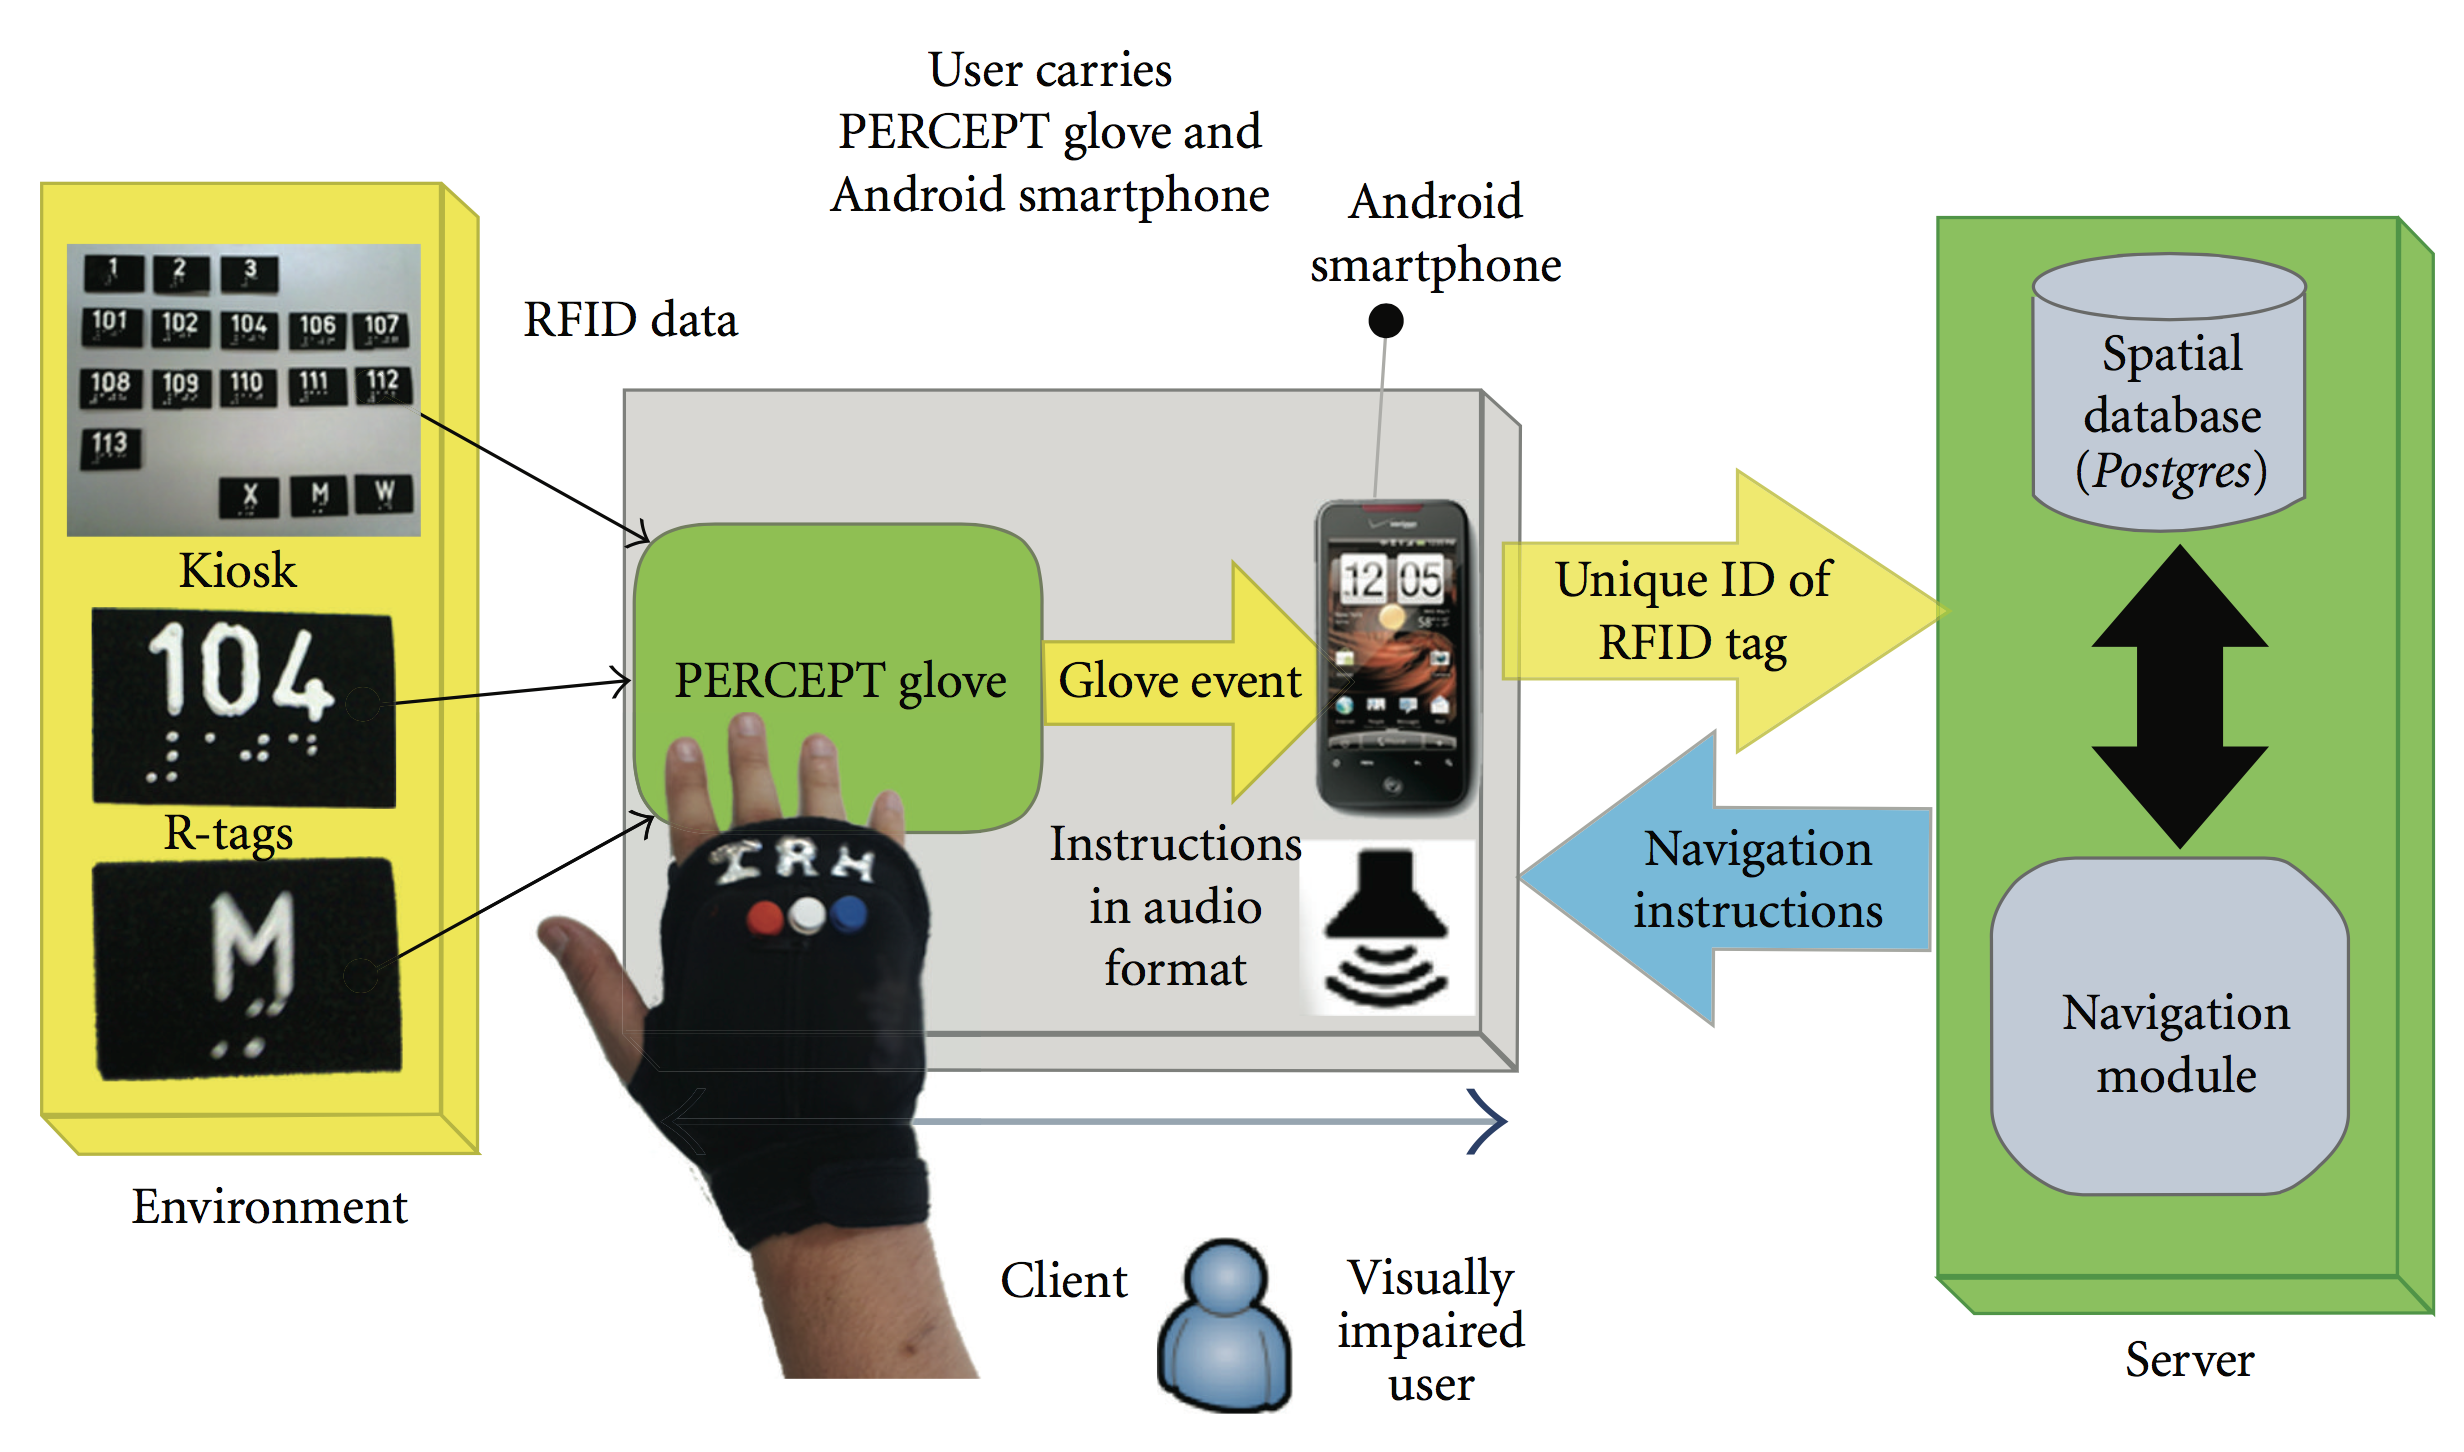
\includegraphics[width=\textwidth]{imgs/perceptArquitetura}
		\fonte{\citetexto{Ganz2011}}
	\end{minipage}
\end{figure}


Em uma breve avaliação do modelo, podemos ressaltar que, devido ao baixo custo das tags RFID, é fácil implantar o sistema em um grande ambiente. Porém, a necessidade de conexão constante com a internet pode ser um problema. Outro ponto bastante problemático é o uso de tags, pois, conforme \citetexto{yang2011supporting}, não é possível assumir que PDV consigam facilmente encontrar tags RFID, por isso muita energia seria para leitura a distância. O fato de o usuário necessitar procurar os quiosques, bem como encontrar a tag correspondente ao destino desejado, é um grande complicador.

%=======================================================================
% UCAT
%=======================================================================
	\section{UCAT - Ubiquitous Context Awareness Tools for the Blind}
\citetexto{ucat2014} apresenta uma pesquisa cujo objetivo é identificar as necessidades de informação de um deficiente visual, focando principalmente em questões relacionadas a percepção, orientação em ambientes conhecidos e desconhecidos e também em dificuldades comumente enfrentadas no dia-a-dia, após algumas entrevistas com PDV o trabalho descobriu que a falta de conhecimento a respeito das pessoas ao redor foi apontada como a principal causa de desconforto. Além disso, todos os entrevistados afirmaram que seria muito bom possuir uma ferramenta sutil e discreta que os ajudasse a obter mais informações sobre seus arredores.

O autor afirma que não existe nenhum sistema que forneça a usuários cegos informações sobre o contexto ao seu redor e propõe um modelo com essa finalidade. Desenvolvido para dispositivos móveis que suportam a tecnologia Bluetooth, objetiva ser uma ferramenta através da qual os PDV podem criar, compartilhar e receber informações a respeito de pessoas, locais ou objetos através de notas. 

Usando Bluetooth como ferramenta de detecção e o endereço MAC do dispositivo para identificar unicamente cada telefone, a aplicação mostra todos os dispositivos ao redor do usuário, sendo capaz de detectar quando alguém se aproxima ou se afasta. O sistema permite criar contatos, associando aparelhos de telefone a pessoas específicas, permitindo também que o usuário crie notas de texto ou voz relacionadas a alguém ou algum lugar. O modelo periodicamente busca por dispositivos próximos e, quando encontra algum, procura se alguma nota foi criada e associada a ele. Se uma associação é encontrada, o aplicativo notifica o usuário através de alertas vibratórios que podem ser personalizados.

Aqui existe um grande ponto fraco da tecnologia utilizada. Para funcionar corretamente, é necessário que todos os dispositivos estejam com o Bluetooth conectado e em modo visível aos demais; caso contrário, o aplicativo é incapaz de detectá-los.

A arquitetura do sistema possui estrutura cliente-servidor, onde o servidor é responsável apenas por hospedar a base de dados e trocar informações entre usuários através da ferramenta Google Cloud Messaging (GCM) \footnote{Ferramenta de mensageria do Google, para mais informações consultar a documentação da ferramenta em https://developer.android.com/google/gcm/index.html} que é usada quando um usuário decide compartilhar alguma informação com outros. O smartphone é o responsável pela execução da maior parte das funcionalidades do modelo. Nele, ficam armazenadas as informações pessoas de cada usuário, seus contatos, associações e notas criadas.

A Figura \ref{fig:visaoGeralUCAT} exibe uma visão geral da arquitetura do modelo UCAT. Nela podemos ver que os clientes conectados ao servidor e ao GCM, enquanto a base de dados se conecta ao servidor e ao GCM. 

\begin{figure}[!ht]
	\caption{Visão geral da arquitetura do UCAT}
	\label{fig:visaoGeralUCAT}
	\centering%
	\begin{minipage}{.6\textwidth}
		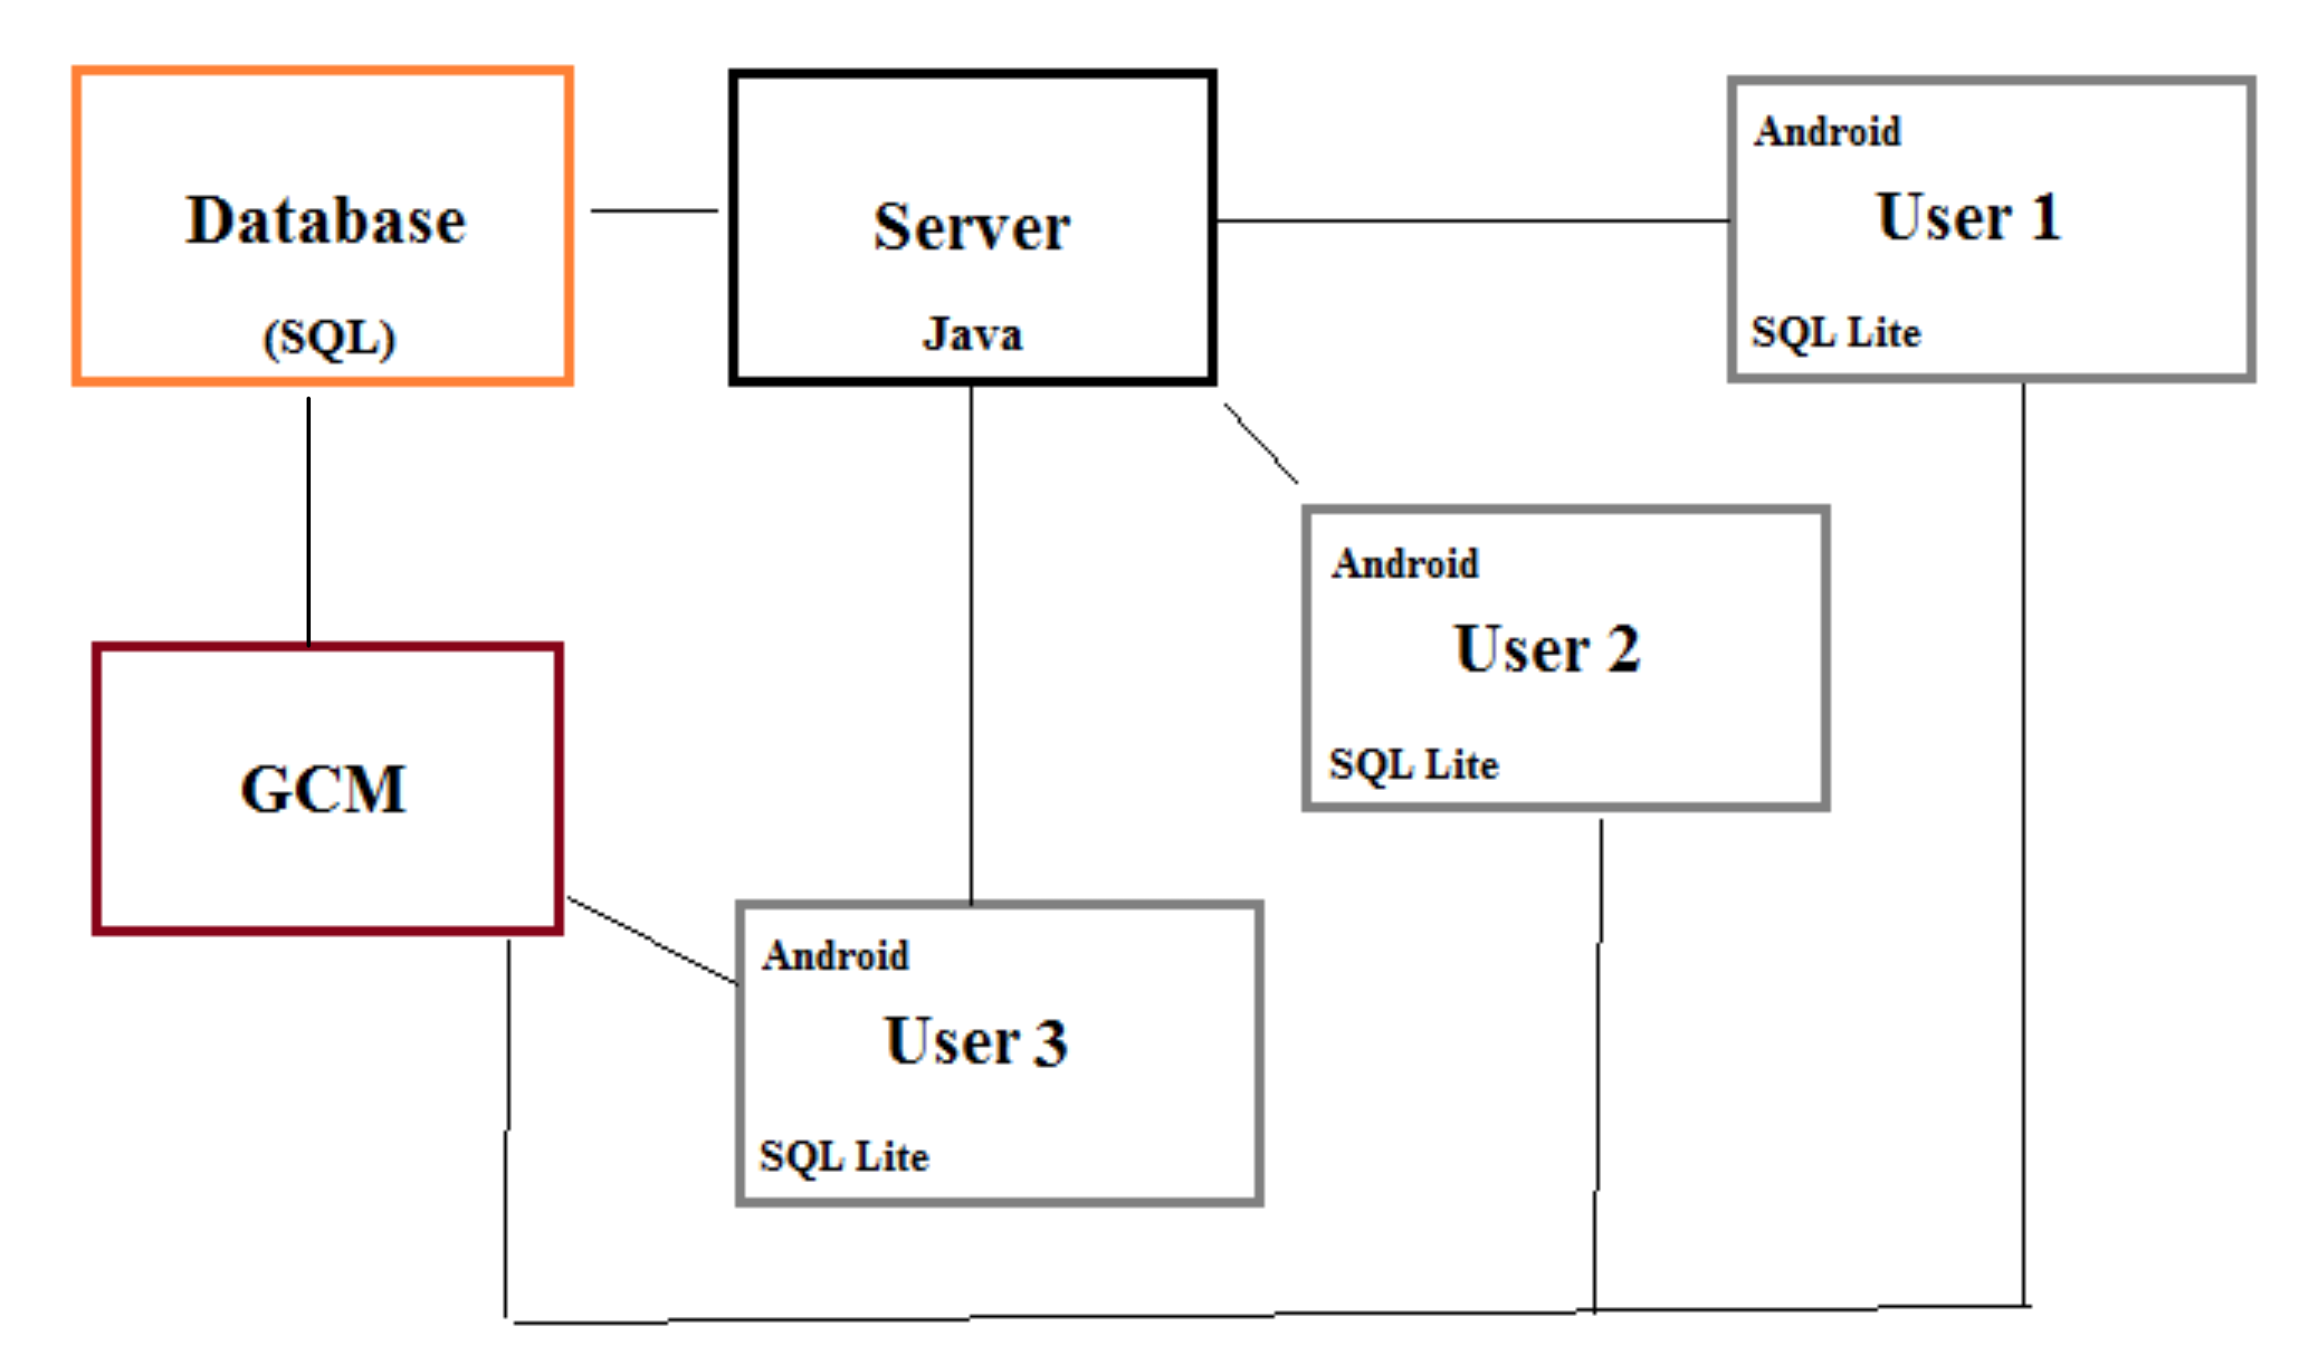
\includegraphics[width=\textwidth]{imgs/ucatArquitetura}
		\fonte{\citetexto{ucat2014}}
		\end{minipage}
\end{figure}

Para facilitar a interação dos usuários com o telefone, o sistema lança mão de alguns recursos de acessibilidade:
\begin{itemize}
	\item O sistema oferece diferentes formas de navegação baseada em gestos realizados na tela, a fim de simplificar a navegação do usuário pelas telas e menus. Alguns gestos disponíveis são o deslizar, o clique duplo e o clique longo. O primeiro tem a função de percorrer as listagens de recursos e menus do aplicativo baseado na direção deslizada na tela. Já os outros servem para confirmar ações ou obter mais informações, respectivamente.
	
	\item Feedback por áudio, ou retorno do sistema através de voz, acontece através da função de conversão de texto para voz nativa do Android\footnote{Mais informações no Centro de Ajuda sobre acessibilidade do Android, em https://support.google.com/accessibility/android/}, sendo empregado para avisar ao usuário em que parte da aplicação ele se encontra, bem como listar funcionalidades de cada tela.

	\item Feedback tátil, ou alertas vibratórios, faz com que cada tipo de notificação emitida pelo sistema seja acompanhada por um padrão diferente de vibração, de modo a permitir que o usuário entenda o motivo do alerta sem obrigá-lo a retirar o telefone do bolso.
\end{itemize}

%=======================================================================
% BLUETOOTH WORKZONES
%=======================================================================
	\section{Development of a Navigation System Using Smartphone and Bluetooth Technologies to Help the Visually Impareid Navigate Work Zones Safely} 

O estudo realizado por \citetexto{chen2014} revela que pedestres correspondem a 17\% das mortes em canteiros de obras nos Estados Unidos. Segundo o autor, um grande planejamento é feito para acomodar o trafego de pedestres ao redor de zonas em obras, especialmente para os deficientes visuais, e garantir segurança no trajeto. O trabalho descreve seus objetivos da seguinte forma: compreender quais as informações relevantes para redirecionar PDV ao redor de obras, a fim de prover mensagens relevantes e criar um sistema para dispositivos móveis com a finalidade de antecipadamente alertar seus usuários sobre a aproximação dos canteiros de obra. Ainda é citada a intenção de padronizar o formato de mensagens emitido em zonas em construção no redirecionamento dos transeuntes, para garantir aos PDV a possibilidade de caminhar independentemente e com segurança.

Para atingir o primeiro objetivo, foram conduzidas entrevistas com PDV com o objetivo de compreender os desafios que eles enfrentam e quais são consideradas informações relevantes durante seu deslocamento. Para o segundo objetivo, o trabalho propõe um aplicativo para smartphones Android que verbalmente emite mensagens enquanto seu usuário se aproxima das áreas delimitadas, fazendo uso de GPS, Bluetooth, função de conversão texto para voz e sensores presentes no telefone. 


\begin{figure}[!ht]
	\caption{Visão geral da arquitetura do modelo}
	\label{fig:visaoGeralWorkzones}
	\centering%
	\begin{minipage}{.6\textwidth}
		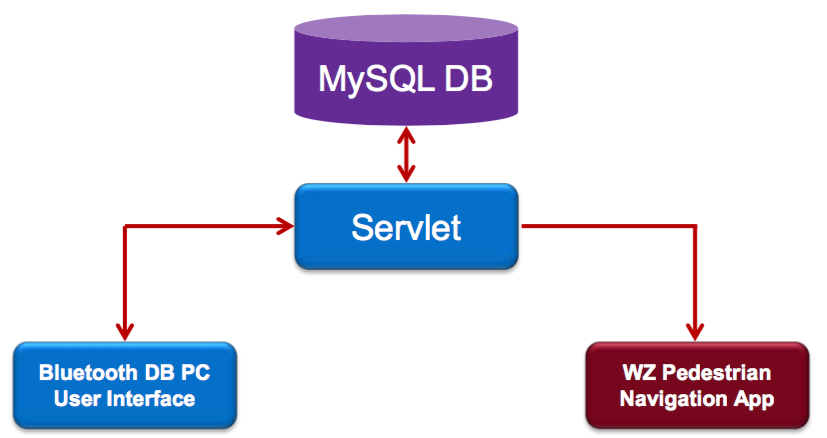
\includegraphics[width=\textwidth]{imgs/workzoneArquitetura}
		\fonte{\citetexto{chen2014}}
		\end{minipage}
\end{figure}


O modelo consiste em três componentes: servidor com banco de dados com mapas, aplicativo para Android e beacons Bluetooth:
\begin{itemize}
	\item O servidor contém o banco de dados onde ficam armazenados os mapas para referência espacial, informações sobre o posicionamento dos beacons e mensagens correspondentes a cada um deles. Essas informações são inseridas no banco de dados através de uma interface web acessada de um computador comum. O modelo de dados de cada beacon compreende um identificador único, latitude, longitude e nome do ponto onde ele foi posicionado e também quatro possíveis textos livres, de acordo com a estrutura das mensagens.

	\item O aplicativo constantemente busca por sinais Bluetooth nas proximidades do usuário. Quando algum é encontrado, seu identificador é comparado com aqueles cadastrados na base de dados espacial. Caso o aplicativo detecte que o usuário se encontra próximo a uma zona em obras, o telefone vibra e o alerta correspondente é emitido verbalmente através da função Text to Speech (TTS) do Android. É também função do aplicativo conectar-se periodicamente ao banco de dados a fim de sincronizar sua base de dados local, mantendo as informações atualizadas. Apenas zonas num raio de até oito quilômetros do usuário são possíveis para garantir o funcionamento mesmo durante um breve período sem conexão com a base.
	
	\item Utilizados devido a possíveis problemas com o sinal GPS fraco ou inexistente, os beacons Bluetooth Smart podem ser posicionados nos limites das zonas em obras, em cavaletes ou cones, conforme mostrado na Figura \ref{fig:workZoneScheme}. São dispositivos de baixo consumo que constantemente emitem seu identificador em um raio de dez metros, podendo ainda ser aumentado ou diminuindo conforme a necessidade.
\end{itemize}

A Figura \ref{fig:visaoGeralWorkzones} mostra a arquitetura do modelo. Nela é possível ver que a base de dados é exposta através de um servidor, sendo acessada pelo aplicativo para obter as informações e por uma outra interface através de uma página web usada para manter as informações.


\begin{figure}[!ht]
	\caption{Demonstração da disposição dos beacons ao redor de uma zona em obras}
	\label{fig:workZoneScheme}
	\centering%
	\begin{minipage}{.4\textwidth}
		\includegraphics[width=\textwidth]{imgs/workzoneSchema}
		\fonte{\citetexto{chen2014}}
		\end{minipage}
\end{figure}


As mensagens emitidas pelo aplicativo seguem o padrão estabelecido durante as entrevistas, sendo formadas por quatro partes distintas \cite{chen2014}:
\begin{itemize}
	\item Breve anúncio para chamar atenção do usuário
	\item Localização atual
	\item O que e onde
	\item Ação recomendada
\end{itemize}

Uma mensagem de exemplo, seguindo esse padrão, poderia ser: Atenção, você está na esquina da Rua X com a Rua Y, a calçada encontra-se fechada por Z metros. Atravesse a rua X para receber mais informações.

O pronto fraco desse trabalho é a baixa área de abrangência da solução, funcionando apenas no entorno de zonas em obras.
A pesquisa e a tecnologia seriam melhores aproveitadas em situações mais corriqueiras, como em um ambiente de uma universidade ou um estádio. Vale citar como ponto forte o uso da última versão da tecnologia Bluetooth, ao contrário dos outros trabalhos citados, onde não é necessário parear os dispositivos para que eles se comuniquem.

%=======================================================================
% TIRÉSIAS
%=======================================================================
	\section{Tirésias}
Em \citetexto{Falk2013} é proposto um modelo para acessibilidade chamado Tirésias. De acordo com o artigo, o Tirésias é baseado no Hefestos. Este, por sua vez, é um modelo genérico que visa estabelecer alguns padrões de acessibilidade que possam ser aplicados em diversos tipos de deficiência. Segundo os autores, o Tirésias pode ser compreendido como uma especialização construída em cima do modelo Hefestos para atender as necessidades das pessoas com deficiência visual. 

De acordo com \citetexto{Falk2013}, o Tirésias emprega conceitos de sensibilidade ao contexto e acessibilidade ubíqua, utilizando maneiras especializadas de interação com o sistema, para promover acessibilidade a PDV. Dessa forma, o modelo é capaz de oferecer informações relevantes ao contexto onde o usuário está e o que existe a sua volta.

O Tirésias funciona obtendo informações de localização do usuário através do GPS contido no smartphone e, baseado nisso, o sistema exibe recursos de acessibilidade disponíveis nas proximidades do usuário. Algumas das funcionalidades oferecidas são a listagem de recursos disponíveis, a indicação de caminho até recurso selecionado e a solicitação de ajuda.

O modelo Tirésias é composto pelos módulos de saída, entrada, configurações e pelo assistente pessoal, somados ao modelo Hefestos. A Figura \ref{fig:visaoGeralTiresias} exibe uma visão geral da arquitetura do Tirésias, mostrando em cima os componentes do próprio modelo, e embaixo os componentes do modelo em que ele é baseado. Os componentes são descritos abaixo.

\begin{figure}[!ht]
	\caption{Visão geral da arquitetura do Tirésias}
	\label{fig:visaoGeralTiresias}
	\centering%
	\begin{minipage}{.6\textwidth}
		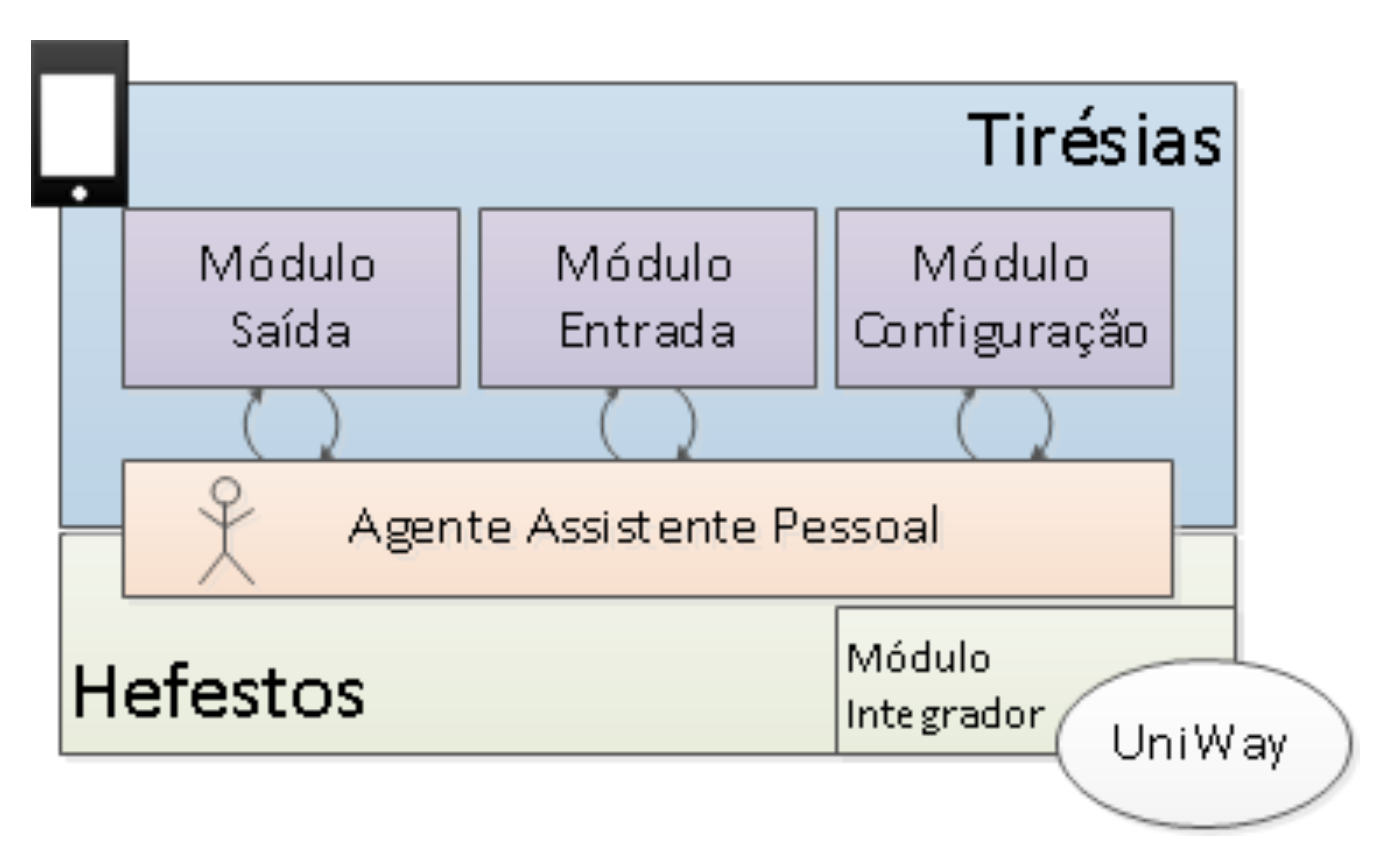
\includegraphics[width=\textwidth]{imgs/tiresiasArquitetura}
		\fonte{\citetexto{Falk2013}}
		\end{minipage}
\end{figure}

\begin{itemize}
	\item O módulo de saída é o responsável por gerenciar as informações passadas aos usuários. Informações são divididas em dois grupos: o primeiro são indicações de recursos disponíveis próximos ao usuário; o segundo tipo são os trechos do caminho até um determinado destino escolhido pelo usuário. Para comunicar as informações ao usuário, são utilizados a leitura da tela em conjunto com alertas vibratórios. A disponibilização das informações do primeiro tipo envolve a leitura do nome, da descrição e da distância até cada recurso um dos recursos disponíveis, baseado na posição atual do usuário. Conforme o usuário se movimenta, a informação de distância dos recursos é atualizada. A diferença do segundo tipo é que apenas o destino parcial mais próximo é disponibilizado e, quando o usuário conclui o trecho atual, o próximo é lido. Além da leitura de tela, o Tirésias combina a utilização de alertas vibratórios com a bússola eletrônica que equipa os smartphone para indicar a direção correta aos usuários. Quando o smartphone está voltado em direção do próximo destino, o fato é informado ao usuário através de vibrações, interrompidas quando o smartphone é virado para outras direções.

	\item O módulo de entrada gerencia a interface do usuário com o sistema. Capaz de suportar dispositivos com teclado dedicado ou somente a tela sensível ao toque, o Tirésias se adapta aos recursos disponíveis no smartphone para oferecer a maneira mais conveniente de interação ao usuário. É através deste módulo que o usuário informa ao modelo onde deseja ir, por exemplo.

	\item O módulo de configuração disponibiliza o controle de ajustes de todas as funcionalidades disponíveis no sistema, de forma a customizar o sistema às necessidades de diferentes usuários. Alguns dos ajustes disponíveis são o controle de frequência e volume da leitura de tela, a quantidade de recursos lida e se o usuário deseja ser notificado quando há alguma mudança nos recursos.

	\item O agente é responsável pela comunicação com o Hefestos, através da qual são obtidos perfis de usuários e recursos disponíveis para o suporte à acessibilidade.
\end{itemize} 

Avaliando o modelo, é notável a acessibilidade no que tange a entrada e saída dos dados no aplicativo. Entretanto, um ponto fraco é a utilização do GPS como modo de localização, visto que o sistema é incapaz de identificar um andar específico em um prédio com muitos pisos, por exemplo, bem como o sinal pode ser fraco ou estar indisponível em algumas regiões devido à natureza da tecnologia. 

	\section{Comparação entre os trabalhos estudados}\label{comparacaoTrabs}

Com o intuito de facilitar a compreensão e a comparação dos trabalhos relacionados, um comparativo entre os trabalhos foi traçado. A partir do comparativo, a Tabela \ref{tab:trabalalhosRelacionados} foi desenvolvida, contendo os principais dados sobre os modelos estudados. Nela são apresentadas as abordagens usadas em cada um dos modelos, sendo possível identificar de forma ágil as características e tecnologias aplicadas em cada um, permitindo a identificação de pontos fortes e lacunas relevantes para o presente trabalho. 

Alguns critérios foram selecionados para uma comparação mais clara entre os trabalhos, cada item da tabela se relaciona com um critério considerado nos modelos selecionados: o método de localização diz respeito a tecnologia utilizada pelo modelo para obter a localização do usuário; a abrangência se refere ao tipo de ambiente em que o modelo se propõe a funcionar; ambientes dinâmicos informa a capacidade do modelo de lidar com mudanças no ambiente; meio de acesso descreve que tipos de hardware são necessário para utilizar o modelo; interface do utilizador descreve as formas usadas pelo usuário para interagir com o modelo; hardware específico indica se o modelo exige que o usuário carregue consigo mais um equipamento ou se o modelo se encaixa em um equipamento já existente; comunicação descreve a maneira utilizada pelo modelo para se comunicar com servidores ou atores externos; interoperabilidade mostra se o modelo prevê que seus dados possam ser utilizados por outras aplicações; banco de dados, linguagem e sistema operacional descrevem quais tecnologias são usadas pelo modelo durante seu desenvolvimento e uso; hardware diz especificamente qual o aparato que o usuário deverá possuir para utilizar o modelo; por fim, arquitetura descreve os componentes de software do modelo e a forma com que eles se comunicam.

Os aspectos mais relevantes na comparação são o meio de acesso utilizado no modelo, a tecnologia aplicada na determinação da localização do usuário, a interface do utilizador e a área de abrangência do sistema. Todos os modelos estudados são focados no uso de dispositivos móveis, no entanto, um deles exige o uso combinado de outro dispositivo de hardware dedicado. Dois dos trabalhos utilizam Bluetooth para obter a localização, enquanto os outros usam RFID ou GPS. Em relação ao último aspecto, três dos sistemas possuem foco em ambientes internos, enquanto um é mais específico e voltado a zonas em construção.


\begin{table}
	\caption{Tabela comparativa entre os trabalhos relacionados}
	\label{tab:trabalalhosRelacionados}
	\centering%
	\begin{minipage}{1\textwidth}
		\begin{adjustbox}{max width=\textwidth}
		\begin{tabular}{ p{3cm} | p{3cm} | p{3cm} | p{3cm} | p{3cm} }
 	\hline
 	& Percept & UCAT & Navigation System for Workzone & Tirésias \\ \hline
	Método de localização & RFID & Bluetooth 2.1 & Bluetooth LE & GPS \\ \hline
	Abrangência & Indoor & Indoor e outdoor & Zonas em obras & Outdoor \\ \hline
	Ambientes dinâmicos & Não especificado & Não especificado & Não especificado & Não especificado \\ \hline
	Meio de acesso & Dispositivos móveis & Dispositivos móveis & Dispositivos móveis & Dispositivos móveis \\ \hline
	Interface do utilizador & Toques & Toques e gestos & Toques & Toques e gestos \\ \hline
	Hardware específico & Sim & Não & Não & Não \\ \hline
	Comunicação & Internet ou intranet & Internet & Internet & Internet ou intranet \\ \hline
	Interoperabilidade & Não & Não & Não & Sim, através de agentes \\ \hline
	Adaptação & Não & Sim, através de sensibilidade ao contexto & Não & Sim, através de sensibilidade ao contexto \\ \hline
	Banco de dados & Postgres & SQLite & MySQL & Não especificado \\ \hline
	Linguagem & Java & Java & Java & Objective-C \\ \hline
	Sistema operacional & Android & Android & Android & iOS \\ \hline
	Bibliotecas utilizadas & Não especificado & Não especificado & Não especificado & Não especificado \\ \hline
	Hardware & Luva equipada c/ leitor RFID e dispositivo móvel c/ Bluetooth & Dispositivos móveis c/ Bluetooth & Dispositivos móveis c/ Bluetooth & Dispositivos Móveis c/ GPS \\ \hline
	Arquitetura & Cliente-servidor & Cliente-servidor & Cliente-servidor & Cliente-servidor \\ \hline
		\end{tabular}
		\end{adjustbox}
		\fonte{Elaborado pelo autor.}
	\end{minipage}
\end{table}


No que tange a outros aspectos avaliados, a arquitetura de todos os modelos se assemelha no uso da estrutura cliente-servidor com comunicação via internet. Apenas o Tirésias foi desenvolvido em Objetive-C para a plataforma iOS, enquanto todos os outros foram desenvolvidos em Java para a plataforma Android. Ainda é possível ressaltar que apenas o Tirésias concebe interoperabilidade para outras aplicações que podem vir a ser desenvolvidas.

Foi identificado que nenhum dos modelos selecionados faz uso de bibliotecas ou frameworks que visem promover acessibilidade. Além disso, as tecnologias de localização usadas em três dos modelos não se adequam perfeitamente a ambientes internos, pois exigem proximidade muito grande do usuário para obter as informações ou então não são capazes de identificar múltiplos andares em um ambiente. O modelo destinado a áreas em construção é o único que faz uso da tecnologia mais adequada, o Bluetooth Low Energy. Porém, a emprega em uma área de abrangência muito pequena.
Outra lacuna identificada foi a falta de informações a respeito do gerenciamento, por parte dos modelos, de mudanças que possam acontecer eventualmente nos ambientes, ou ambientes dinâmicos. Por fim, foi identificado que o único modelo que considera a possibilidade integração com outras soluções é o Tirésias.

%=======================================================================
% Modelo proposto
%=======================================================================
\chapter{Modelo Proposto}
% Essa etapa consiste em detalhar o modelo. O capítulo do modelo deve começar a partir da delimitação da pesquisa, dizendo quais lacunas serão atacadas e como. Geralmente há uma visão geral do modelo aqui, já desenvolvido na atividade 4. Esse capítulo detalha como a questão de pesquisa será respondida? Que modelo computacional é necessário para isso. Se é proposta uma ontologia, ela é detalhada aqui; Se há um modelo de contexto, ele é detalhado aqui. Pode-se usar alguns diagramas para representar a arquitetura, interações, fluxos e componentes. Lembre-se que o modelo pode ter diferentes implementações e não precisa ser limitado por uma tecnologia específica. Por exemplo, não faz sentido dizer que o modelo é para Android ou feito em Java. Por que não poderia ser para iOS e feito em Objective C? Que característica de um modelo limitaria isso?

% Lacunas
% Visão geral
% Como a questão de pesquisa será respondida
% Diagramas (arquitetura, interações, fluxos e componentes)

\epigrafecap{For most people, technology makes things easier. \\
For people with disabilities, technology makes things possible.}
{Mary Pat Radabaugh}

Este capítulo apresenta um modelo de sistema que visa promover acessibilidade de pessoas com deficiência visual. O modelo atua auxiliando na localização e no deslocamento de seus usuários, contando com recursos que facilitam sua interação, visto que PDV necessitam de formas especializadas de contato com dispositivos. \citetexto{Falk2013}.

Os principais recursos agregados ao modelo são a utilização de uma arquitetura de serviço na nuvem com servidores distribuídos, uma evolução do modelo cliente-servidor; e também a utilização do framework indoo.rs, criado pela empresa Indoors. \footnote{Para mais informações consultar o site oficial da empresa em http://indoo.rs/solutions/} O indoo.rs promove acessibilidade buscando ser a base na qual são montadas aplicações que necessitam de informações precisas e em tempo real. A decisão de usar essa biblioteca se deve ao fato do framework facilitar o desenvolvimento multiplataforma de soluções de localização através de beacons Bluetooth. Outras características do indoo.rs são a dispensa da necessidade de conexão com a internet, o baixo consumo de energia e a inclusão de ferramentas analíticas e gerenciais, através das quais é possível extrair inúmeras informações a respeito do movimento dos usuários nas premissas do ambiente. Outros diferenciais do modelo são a utilização de sensibilidade ao contexto e o suporte às funcionalidades de acessibilidade, oferecidas nativamente pelos sistemas operacionais.
São previstos também o suporte a ambientes dinâmicos e a possibilidade de integração com outras soluções, ambos através de serviços web.

\section{Visão geral do modelo} 
O modelo, batizado de Insight, foi desenvolvido após análise dos trabalhos científicos relacionados. Deles foram aproveitados conceitos e funcionalidades consideradas essenciais e descartadas ideias consideradas incompatíveis com este trabalho. A arquitetura do cliente Insight é baseada naquela apresentada por \citetexto{Ganz2011}. O emprego da ciência de contexto, apesar de ser fundamentalmente diferente, e a metodologia de avaliação são inspirados pelo apresentado em \citetexto{Falk2013}, juntamente com a ideia de expor os dados da solução para serem consumos por soluções de terceiros. A estruturação das mensagens e a sincronização entre cliente e serviço são conceitos apresentados em \citetexto{chen2014}. Os feedback auditivo e tátil são utilizados em \citetexto{ucat2014}. Podem ser citadas como exemplos de ideias descartadas a necessidade de hardware dedicado, juntamente com o emprego de uma tecnologia que exige proximidade por parte do usuário, ambas usadas pelo PERCEPT; e o uso da tecnologia GPS, utilizada no Tirésias.

O Insight foi concebido tendo em mente tecnologias existentes e disponíveis ao alcance da maioria das pessoas. Todos os equipamentos necessários já existem no mercado, de forma que não é preciso fazer modificações em produtos para aproveitar as funcionalidades aqui descritas.

O objetivo do modelo é promover acessibilidade aos seus usuários, possibilitando que eles estejam sempre cientes dos locais ao seu redor e do caminho até eles. Para isso, o cliente auxilia o usuário em seu deslocamento curva-a-curva através de instruções verbais. Alguns dos locais que terão sua localização indicadas aos usuários através do cliente são banheiros, balcões de informação, estações policiais, locais preparados para receber deficientes visuais, zonas em obras e pontos de transporte público. Essas informações são caracterizados por \citetexto{stewart2008accessible} como extremamente importantes para os PDV.

Visto que não faz parte do objetivo do modelo alertar sobre obstáculos no caminho do usuário, ele não deve ser encarado como um substituto para ferramentas que possuam esse fim. O Insight deve ser sempre usado em conjunto com outras ferramentas assistivas, tais como bengalas e cães guia, esses sim possibilitam o desvio de obstáculos de qualquer natureza que possam surgir. 

Empresas ou organizações que queiram melhorar a acessibilidade de suas dependências devem ter em mente que outras medidas podem ser tomadas em conjunto com a adoção do modelo, para aumentar a eficiência de seus esforços. Uma medida que possui sinergia total com o Insight é a colocação de piso tátil por todos os trajetos que serão percorridos pelos PDV. Piso tátil são faixas em alto-relevo no chão percebidas pelos usuário através da sensibilidade dos pés, fornecendo auxílio e indicações aos PDV durante seus deslocamentos.

A combinação Insight e piso tátil é bastante útil no empoderamento e independência dos usuários. O Insight permite descobrir locais e rotas, e o piso tátil permite que os usuários tenham certeza de que o caminho sendo percorrido é seguro e não possui obstáculos que dificultem o trânsito.

O modelo é composto por uma aplicação cliente, uma aplicação servidor, pela camada de serviço e diversos beacons Bluetooth, conforme mostrado na Figura \ref{fig:visaoGeral}. 

O cliente contempla os seguintes módulos: interface do usuário, módulo de saída, módulo de sincronização, motor de localização, serviço Bluetooth e uma base local. 
A camada de serviço contém uma ferramenta de gerenciamento dos ambientes, um módulo de controle e todas as instâncias em execução da aplicação servidor. Ela também é chamada de serviço Insight.
Cada instância contém um web service REST, uma base de dados local e um módulo de conexão ao banco de dados. 
Os beacons serão previamente distribuídos em pontos-chave do local onde o modelo for aplicado, de forma a otimizar seu alcance e área de cobertura.

Através do modelo, o usuário poderá saber onde está, descobrir locais que existem a sua volta e selecionar algum recurso específico para que seja traçada uma rota para chegar ao destino escolhido, entre outras funcionalidades. O cliente fornece instruções via áudio e alertas vibratórios, através dos recursos assistivos dos smartphones, para guiar o usuário conforme avança pelo caminho até o seu destino. A Figura \ref{fig:fluxoBasico} mostra o fluxo básico do processo de uso do Insight, desde a escolha do destino, passando pelo deslocamento do usuário até que ele chegue no destino final.

\begin{figure}[!ht]
	\caption{Fluxo básico da execução}
	\label{fig:fluxoBasico}
	\centering%
	\begin{minipage}{.8\textwidth}
		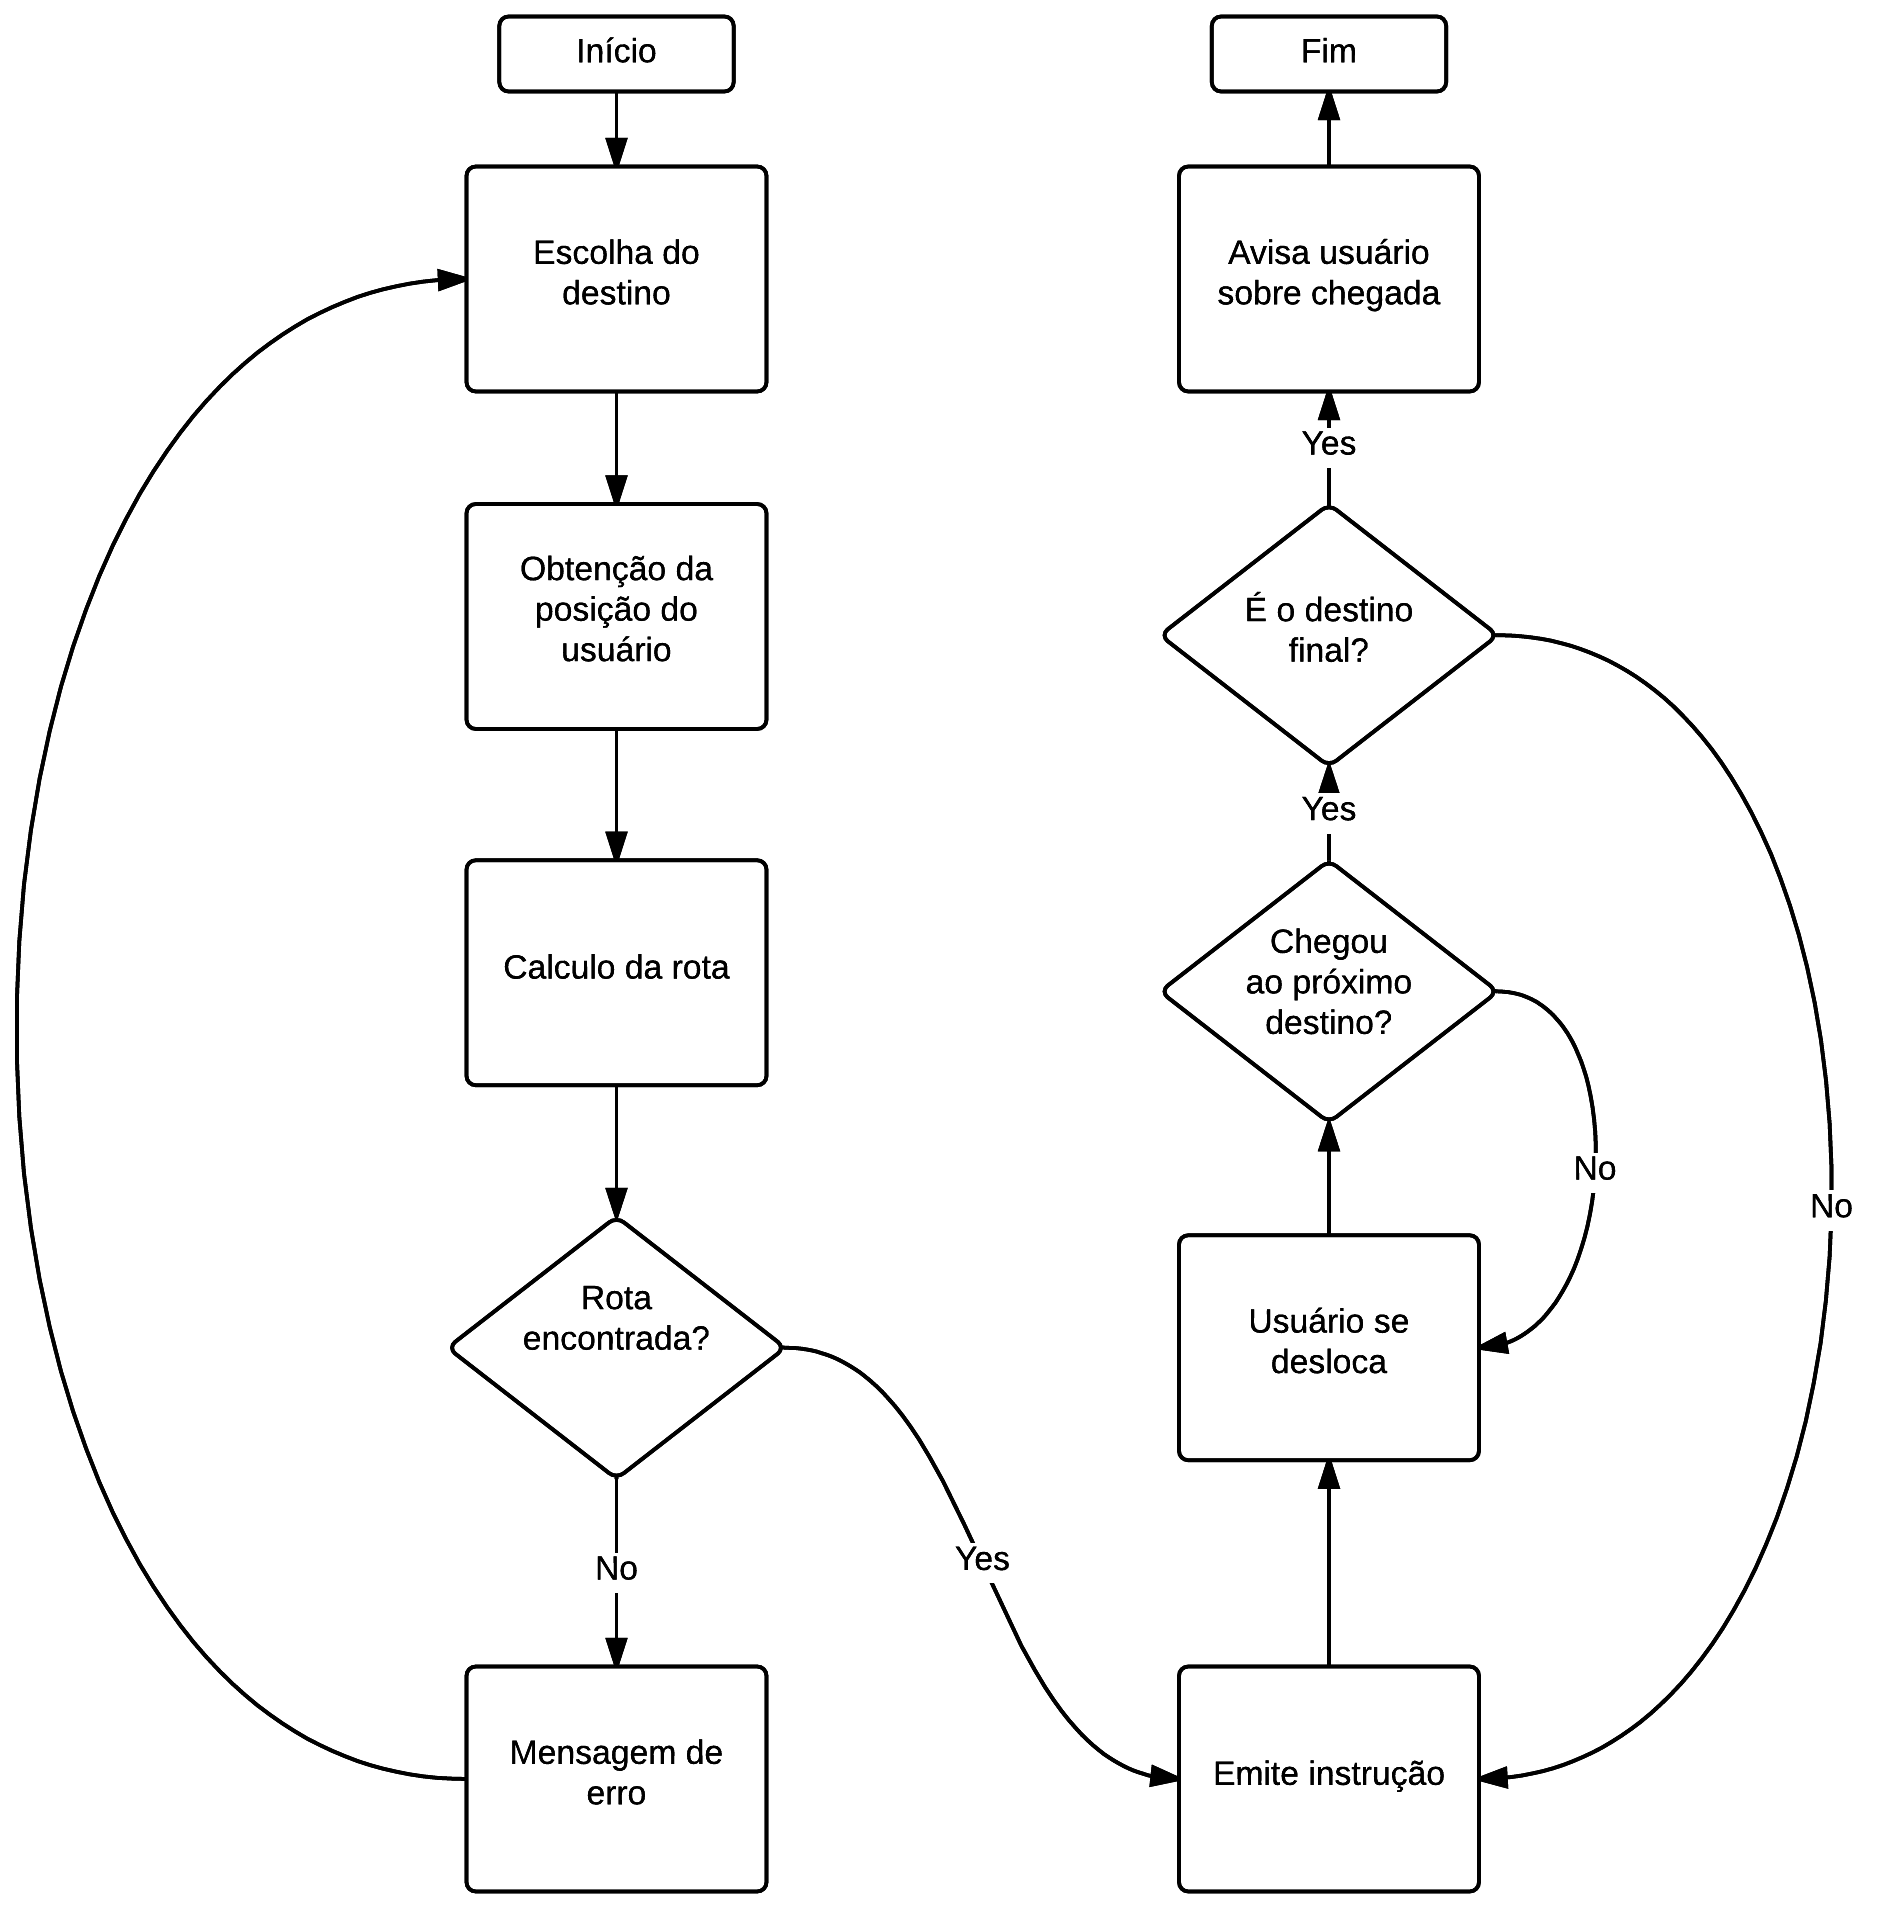
\includegraphics[width=\textwidth]{imgs/fluxoBasico}
		\fonte{Elaborado pelo autor.}
	\end{minipage}
\end{figure}

\citetexto{dias2015navpal} afirma que, quando perdidos ou desorientados, PDV frequentemente requisitam ajuda de pessoas próximas. Como não é objetivo do Insight eliminar completamente a assistência humana e também por precaução, caso o usuário entre em algum ambiente fora do alcance dos beacons, é prevista no modelo a funcionalidade do pedido de ajuda. Quando o usuário a aciona, sua última localização conhecida é enviada pelo modelo para números de telefone cadastrados no modelo. Então os administradores podem providenciar que alguém vá ao encontro de quem necessita de ajuda.

De acordo com \citetexto{gedawy2011designing}, qualquer sistema de navegação destinado a PDV conter cinco elementos essenciais. São eles: uma representação geografia capaz de representar múltiplos andares; uma funcionalidade para calcular as rotas e direções dos usuários; uma maneira de identificar a localização do usuário; uma interface para gerenciar a interação do usuário; e, por último, um componente que traduza as rotas para uma forma de comunicação compreensível pelo usuário. \cite{gedawy2011designing}. O cliente Insight possuí cada um destes elementos.

A arquitetura do modelo, bem como cada um dos componentes, é explicada em maiores detalhes nas seções subsequentes.

\begin{figure}[!ht]
	\caption{Visão geral do modelo}
	\label{fig:visaoGeral}
	\centering%
	\begin{minipage}{.8\textwidth}
		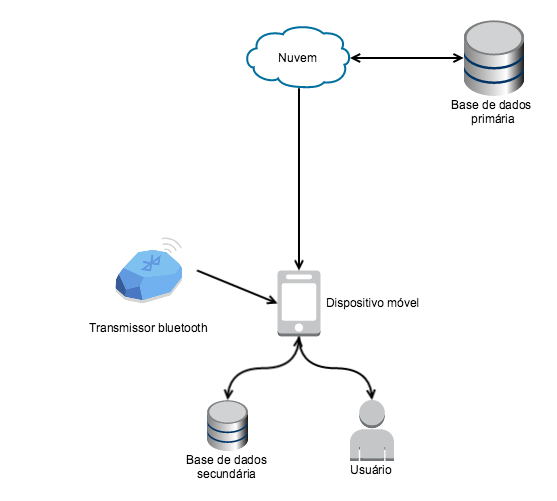
\includegraphics[width=\textwidth]{imgs/visaoGeral}
		\fonte{Elaborado pelo autor.}
	\end{minipage}
\end{figure}

	\section{Arquitetura}
O Insight é projetado para ser um serviço na nuvem com servidores distribuídos. Diversas instâncias da aplicação servidor são executadas simultaneamente para garantir escalabilidade e disponibilidade. Tal arquitetura possui o objetivo de permitir que diversos usuários possam acessar o sistema sem que a performance seja prejudicada. Por sua vez, os clientes são instalados em dispositivos móveis, como smartphones e tablets, e se comunicam com o serviço Insight através de web services REST localizados em cada uma das instâncias. A Figura \ref{fig:arquitetura} mostra um diagrama de blocos onde os principais componentes da arquitetura são exibidos, mostrando também as camadas em que ela está dividida e como ocorre a troca de informações entre os componentes. 


\begin{figure}[!ht]
	\caption{Diagrama de blocos da arquitetura simplificada}
	\label{fig:arquitetura}
	\centering%
	\begin{minipage}{.8\textwidth}
		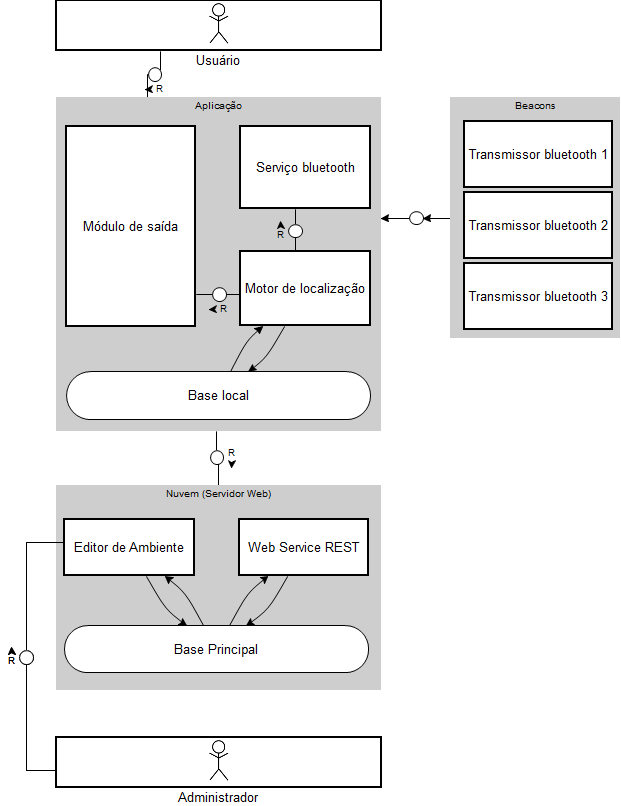
\includegraphics[width=\textwidth]{imgs/arquitetura.png}
		\fonte{Elaborado pelo autor.}
	\end{minipage}
\end{figure}


A Figura \ref{fig:diagramaSequencia} mostra um diagrama de sequência detalhando a troca de mensagens entre os componentes do modelo durante a execução de algumas tarefas no Insight.


\begin{figure}[!ht]
	\caption{Diagrama de sequência do modelo}
	\label{fig:diagramaSequencia}
	\centering%
	\begin{minipage}{.5\textwidth}
		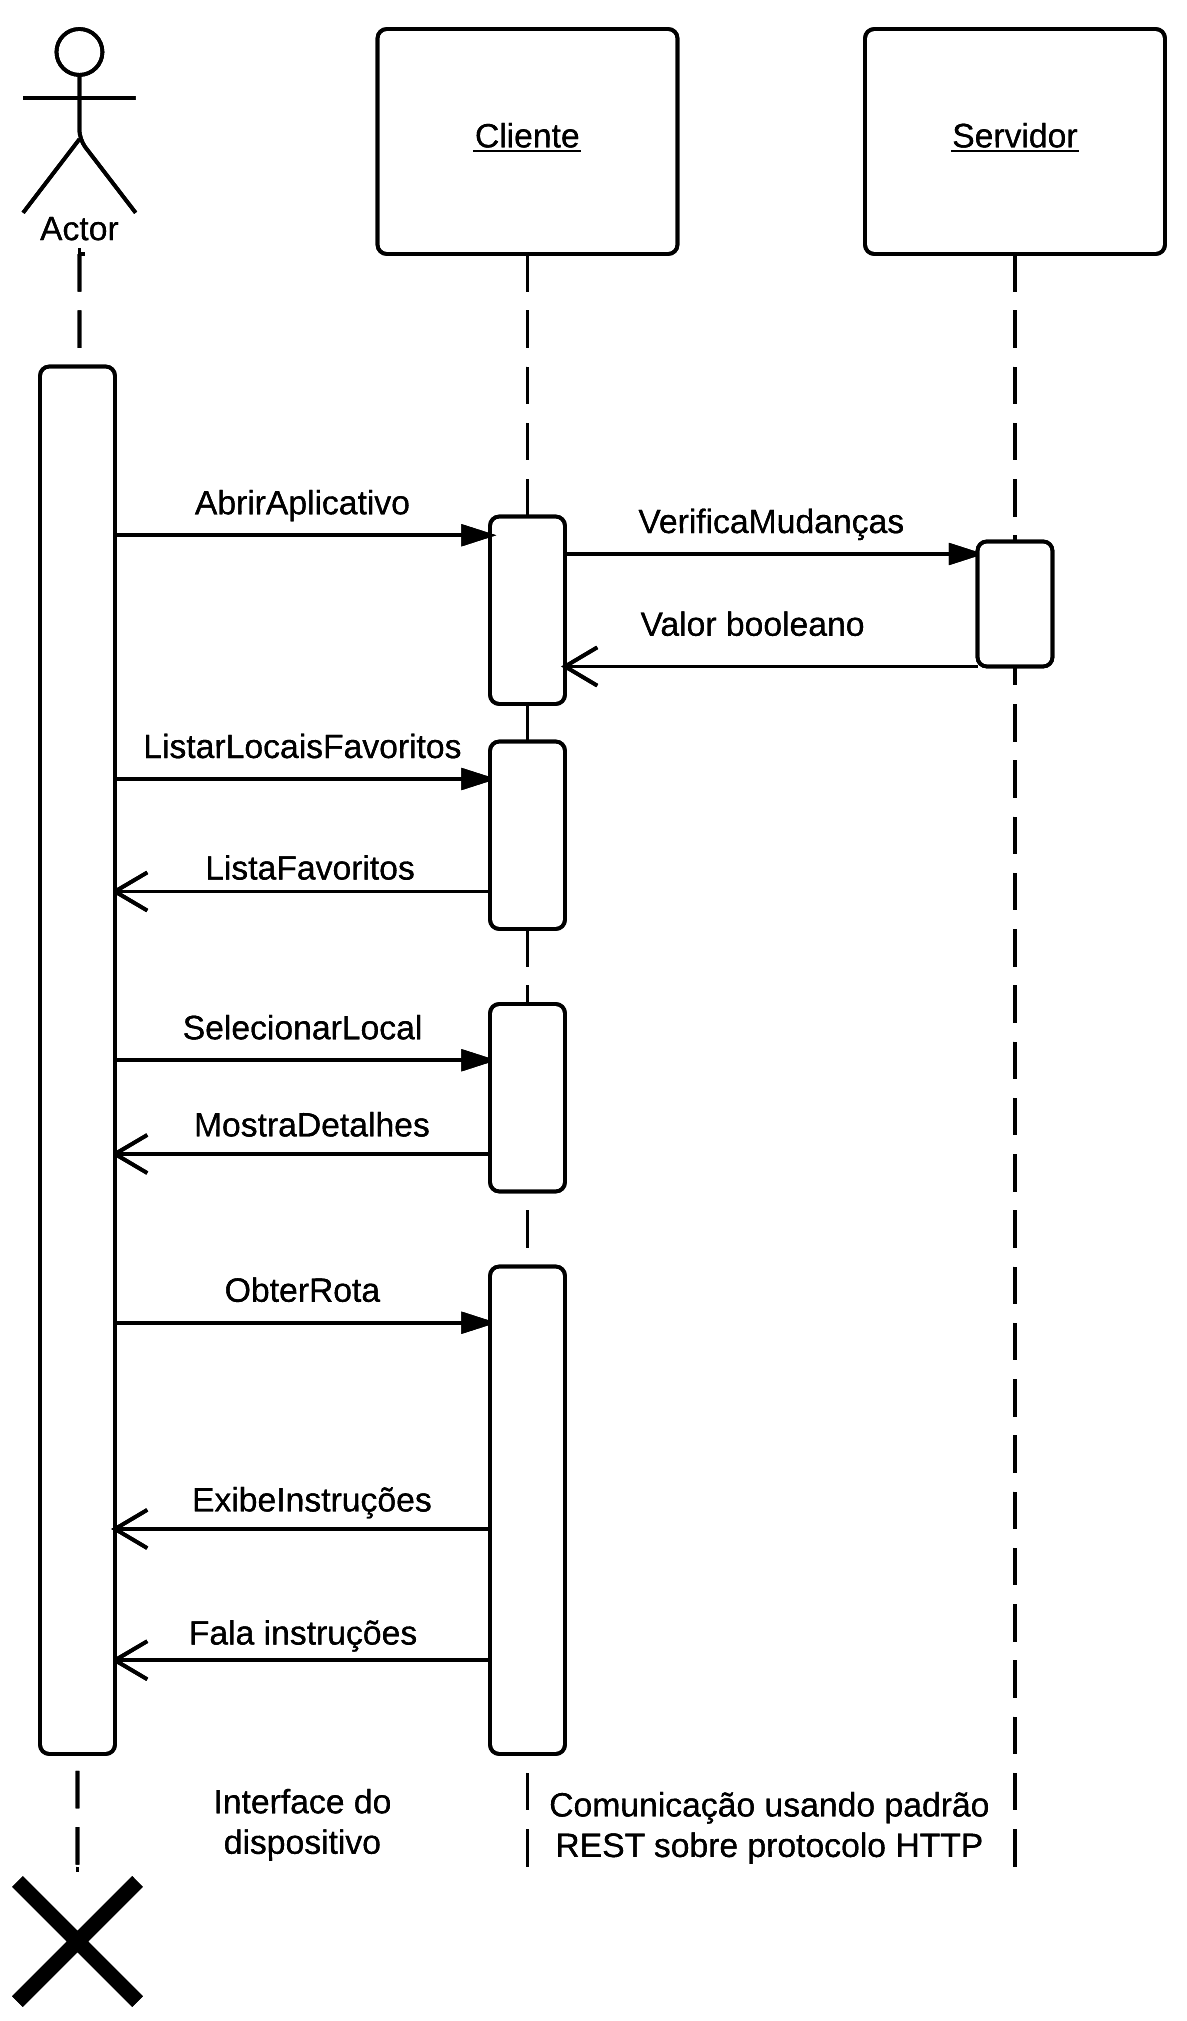
\includegraphics[width=\textwidth]{imgs/diagramaSequencia.png}
		\fonte{Elaborado pelo autor.}
	\end{minipage}
\end{figure}


	\subsection{Componentes do cliente}
Nesta seção são detalhadamente apresentados cada um dos componentes que formam a arquitetura da aplicação para dispositivos móveis do modelo Insight, mostrados na Figura \ref{fig:arquiteturaCliente}.

\FloatBarrier
\begin{figure}[!ht]
	\caption{Diagrama de blocos da arquitetura da aplicação cliente}
	\label{fig:arquiteturaCliente}
	\centering%
	\begin{minipage}{.8\textwidth}
		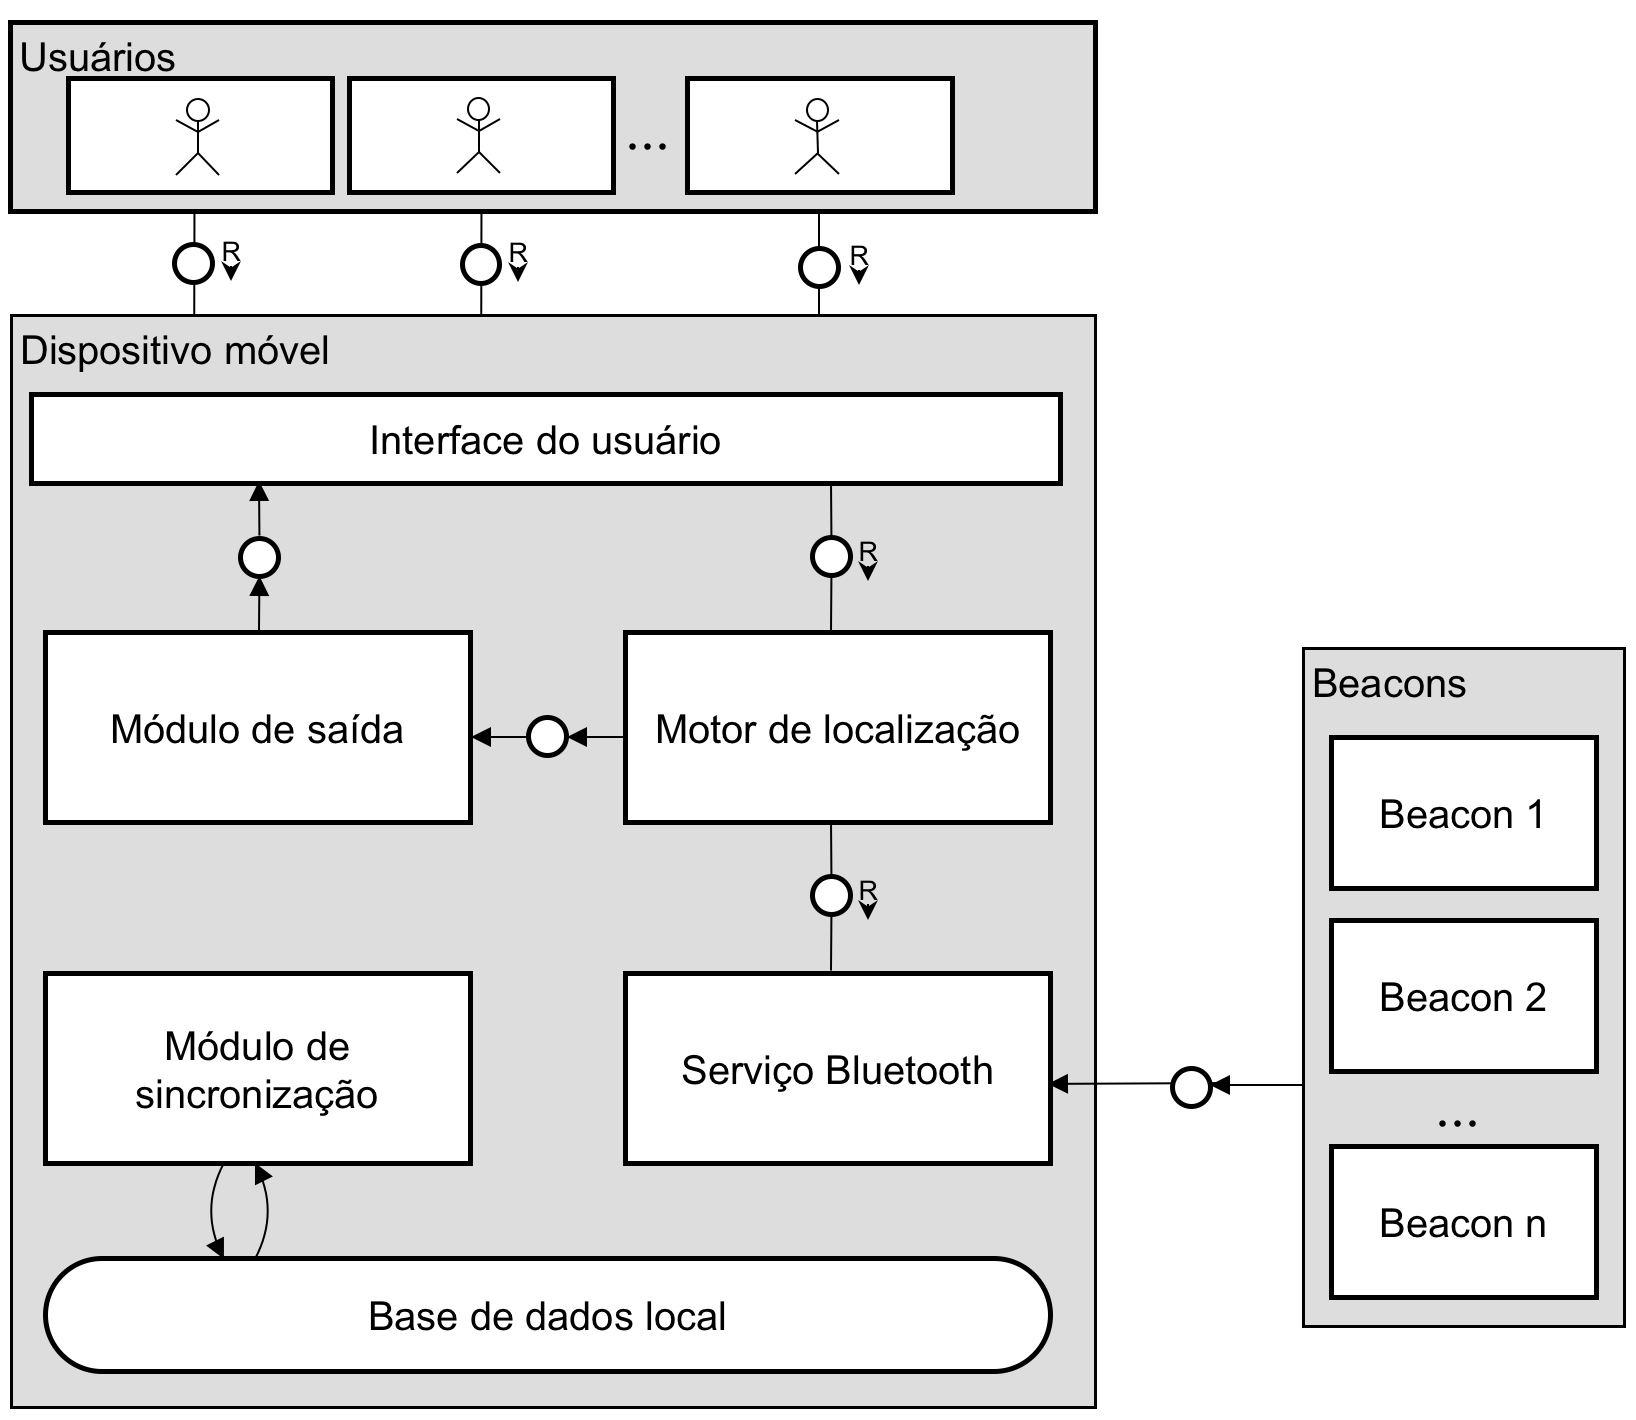
\includegraphics[width=\textwidth]{imgs/arquiteturaCliente.png}
		\fonte{Elaborado pelo autor.}
	\end{minipage}
\end{figure}
\FloatBarrier

		\subsubsection{Módulo de sincronização}
Para que o cliente possa ser usado sem a exigência de conexão constante com a internet existe o módulo de sincronização. Ele é o responsável por manter a base de dados do cliente sempre atualizada em relação a base de dados principal do modelo, localizada nas instâncias, e também enviar as informações de monitoramento do cliente para a nuvem.

O módulo se conecta com a camada de serviço e verifica se existem modificações nos locais ou nos beacons desde a última sincronização e, em caso positivo, copia as novas informações até que as duas bases estejam equiparadas. Por padrão, a verificação em busca de modificações ocorre semanalmente, de forma a não consumir muito da bateria dos dispositivos. Todavia, o administrador pode alterar esse valor para mais ou para menos a fim de permitir que o modelo lide com mudanças dinâmicas no ambiente. A habilidade de suportar mudanças dinâmicas no ambiente é, segundo \citetexto{quinones2011supporting}, uma característica muito importante num sistema de localização acessível, visto que caminhos já conhecidos pelos usuários podem sofrer alterações, mesmo que levemente. Mudanças dinâmicas são alterações não previstas em rotas ou locais, como por exemplo um elevador não funcionando, uma sala fechada para limpeza, um caminho em manutenção, etc.

A execução da sincronização é independente do usuário, sendo realizada de forma automática e transparente, através de uma conexão com o serviço Insight via internet, usando o padrão REST para troca das informações.

		\subsubsection{Base de dados local}
É função principal da base de dados local manter uma cópia das informações do serviço Insight, bem como dados relativos as preferências do usuário. Esses dados ficam armazenados localmente no dispositivo. Exemplos de informações mantidas por esta base são as informações completas referentes aos beacons e locais cadastrados no serviço e também os locais marcados pelo usuário como seus favoritos.

Além da função principal, a base local também guarda informações anônimas que visam permitir uma execução otimizada do cliente, tais como histórico completo de sincronizações realizadas, e dados de monitoramento do cliente, destinos selecionados pelo usuário, como rotas traçadas pelo sistema, instruções dadas ao usuário, informações de tempo e hora de uso, entre outras. Para garantir a privacidade do usuário, todas as informações analíticas do cliente são anonimizadas.

A base local é alimentada pelo módulo de sincronização, responsável por adicionar ou excluir os dados cadastrados. Seu objetivo é aumentar a usabilidade do cliente, não exigindo conexão com a internet para traçar as rotas, tornando mais rápida a resposta ao usuário.

		\subsubsection{Motor de localização}
O motor de localização é, juntamente com o serviço Bluetooth, o coração do modelo. Sua função é combinar as requisições recebidas do usuário com os dados do serviço Bluetooth para então calcular as rotas desde a localização atual do usuário até o destino por ele escolhido. Uma vez que o cliente é ativado, sua localização é obtida e informada ao usuário através do uso de voz.

A rota calculada pelo Insight é comunicada ao usuário de forma a se moldar à maneira com a qual os PDV planejam seu caminho, descrita por \citetexto{harper2000travel}: PDV costumam fragmentar sua jornada em partes menores e mais gerenciáveis, assim podem controlar seu deslocamento por etapas. Conforme \citetexto{quinones2011supporting}, quando o usuário precisa rotineiramente percorrer uma mesma rota ele cria mapas mentais detalhados, afim de memorizar rotas e marcos específicos dos locais por onde passa. 

O Insight, após definir a rotas, a divide trajetos menores e a comunica ao usuário por etapas. Quando o usuário termina de percorrer um trecho ele recebe um novo conjunto de instruções, servindo também como confirmação de que o usuário está no caminho correto. De acordo com \citetexto{Falk2013}, uma definição otimizada da granularidade e da velocidade de leitura das instruções é importante para não sobrecarregar o usuário com instruções demais, podendo deixa-lo confuso e desorientado. 

Para o cálculo das rotas é usado o algoritmo proposto por \citetexto{dijkstra1959note}. O algoritmo de Dijkstra soluciona o problema do caminho de custo mínimo em um grafo cujas arestas não possuem peso negativo, como é o caso das rotas do Insight.

	\subsubsection{Serviço Bluetooth}
O serviço Bluetooth é a parte do cliente onde está toda a programação que o torna compatível com a tecnologia Bluetooth Low Energy. Através dele é feita o monitoramento dos beacons presentes no entorno do usuário, permitindo com que sua localização atual seja obtida.

Este módulo, juntamente com os beacons, fornece o contexto do usuário para o modelo. Através do contexto é possível atuar quando mudanças são identificadas, adaptando as instruções dadas ao usuário conforme ele se desloca, se aproximando ou se distanciando do destino.

Esse módulo é capaz de continuar a atuando mesmo após o bloqueio do smartphone, guiando o usuário através de mensagens verbais. Outra funcionalidade possível através deste componente é detectar quando o usuário adentra no ambiente onde o modelo está implantado, avisando ao usuário sobre sua existência e questionando se ele deseja usar o cliente. Esse comportamento pode ser desativado, caso seja essa a preferência do usuário.

O processo de identificação de um beacon por parte do cliente pode ser resumido como o seguinte:
\begin{itemize}
	\item Beacon transmite seu identificador no ambiente em que está instalado. 
	\item Cliente detecta a transmissão do beacon e determinar o identificador.
	\item Cliente verifica em sua base de dados a localização associada a esse identificador.
	\item Cliente obtém a localização atual do usuário e se adapta ao novo contexto.
	\item Cliente decide se há alguma ação para ser tomada, baseada no contexto do usuário.
	\item Se houver alguma ação, o cliente a executa.
	\item Cliente informa usuário sobre a ação, através de voz ou alertas vibratórios.
\end{itemize}

Uma grande vantagem do uso de beacons é a capacidade de transmitir e receber identificadores sem que seja necessário parear os dispositivos envolvidos. Isso permite que qualquer smartphone que imediatamente identifique e capte o sinal, não exigindo ações por parte do usuário.

Os beacons devem ser espalhados em pontos chave do ambiente e em todos os destinos possíveis. Desta forma é garantida a área de cobertura do modelo e a otimização na quantidade de beacons necessários, fazendo com que o usuário sempre possa descobrir sua localização e sempre possa chegar ao destino desejado. O Insight não exige a posição exata e precisa do usuário, então apenas um beacon é capaz de fornecer a localização necessária. Caso fosse indispensável ter a localização exata seriam necessários pelo menos três beacons por local, possibilitando a triangulação da posição.

	\subsubsection{Interface do usuário e módulo de saída}
A interface do usuário é responsável por gerenciar o trato do usuário com o sistema. O módulo de saída é o responsável pelo feedback dado ao usuário. Estes componentes são profundamente integrados um com o outro. A fim de suportar as necessidades dos PDV, a interface oferece métodos especializados de interação como navegação por gestos e voz, e o módulo de saída oferece feedback através de voz e alertas vibratórios. 
O Insight usa os recursos acessíveis presentes no sistema operacional para modificar drasticamente as formas de interação do sistema. 

O clique simples tem seu efeito modificado. Ao invés de ativar ou abrir, o clique simples apenas seleciona algum item. Para ativar um abrir um item selecionado são necessários dois toques em qualquer parte da tela. Em listas de seleção, como por exemplo a lista de locais próximos ao usuário ou sua lista de locais favoritos, a navegação é feita a partir de gestos. Deslizar o dedo para a direita ou para baixo avança a seleção, já deslizar o dedo para esquerda ou para cima faz a seleção retornar um item. Cada vez que um item é selecionado seu nome é lido para o usuário. Duas formas são previstas para rolar a tela, deslizando dois dedos na direção desejada ou então com um deslize seguido imediatamente por outro na direção contrária. Em telas que possuem componentes variados, como campos de texto e botões, a navegação é ainda mais especializada, lendo não apenas o nome do componente, mas também sua descrição e, quando disponível, seu tipo e estado atual. A navegação entre itens é idêntica a das listas de seleção, deslizando o dedo para baixo ou para a esquerda o próximo componente é selecionado e lido. Por exemplo, se o item selecionado for um botão com o texto "Obter rota" a leitura seria "Obter rota, botão"
Para a inserção de texto o processo é bem similar. O teclado é percorrido com os mesmos gestos citados anteriormente, e cada letra selecionada é lida ao usuário. Para percorrer o texto escrito são usados gestos, e o usuário pode definir a granularidade do deslocamento em letras, palavras, frases ou parágrafos.

\citetexto{mau2008blindaid} compara diversas formas de instruir o usuário PDV durante seu deslocamento. Após comparar instruções faladas, tons, forma de bussola e feedback tátil o trabalho indica que a melhor maneira é mesmo o uso de instruções verbais. Quando um usuário solicita que o sistema calcule uma rota até algum destino, independentemente se foi usada voz ou escrita, as instruções também são passadas pelo Insight verbalmente. Porém, a leitura ocorre de uma maneira um pouco diferente. Conforme \citetexto{ullman2009accommodating}, é importante fornecer instruções claras, citando também elementos espaciais que podem ser usados como referências pelos usuários.

O Insight emite um bipe antes de cada instrução, a fim de chamar a atenção do usuário, o alertando que ele chegou em um novo marco do caminho e uma nova instrução será proferida. Instruções são passadas apenas em pontos chave do trajeto, de forma a evitar que uma frequência muito alta de informações sobrecarregue o usuário. Unidades de medidas de distância como metros são evitadas, preferindo informar o usuário do número aproximado de passos até o próximo destino. As instruções alertam o usuário sobre obstáculos no caminho, tais como escadas, aclives ou declives, caso estes existam.

Todas as falas são geradas por computador. Isso permite economizar o tamanho do software cliente, pois não é necessário armazenar arquivos de áudio, e também responder rapidamente a mudanças no ambiente, visto que não existe a exigência as falas passem por todo o processo de gravação e que o cliente tenha de ser atualizado para ter as novas instruções.	














	\subsection{Componentes do serviço Insight}
Nesta seção são detalhadamente apresentados cada um dos componentes que formam a arquitetura da camada de serviços do Insight, mostrados na Figura \ref{fig:arquiteturaServico}.

A camada de serviço do Insight é composta pela totalidade das instâncias em execução, um módulo de controle, um editor de ambientes e a principal base de dados do modelo. 

O uso do modelo de computação na nuvem permite que o sistema possa ser acessado por um grande número de usuários mantendo baixos custos de infraestrutura.

\FloatBarrier
\begin{figure}[!ht]
	\caption{Diagrama de blocos da arquitetura da camada de serviço}
	\label{fig:arquiteturaServico}
	\centering%
	\begin{minipage}{.7\textwidth}
		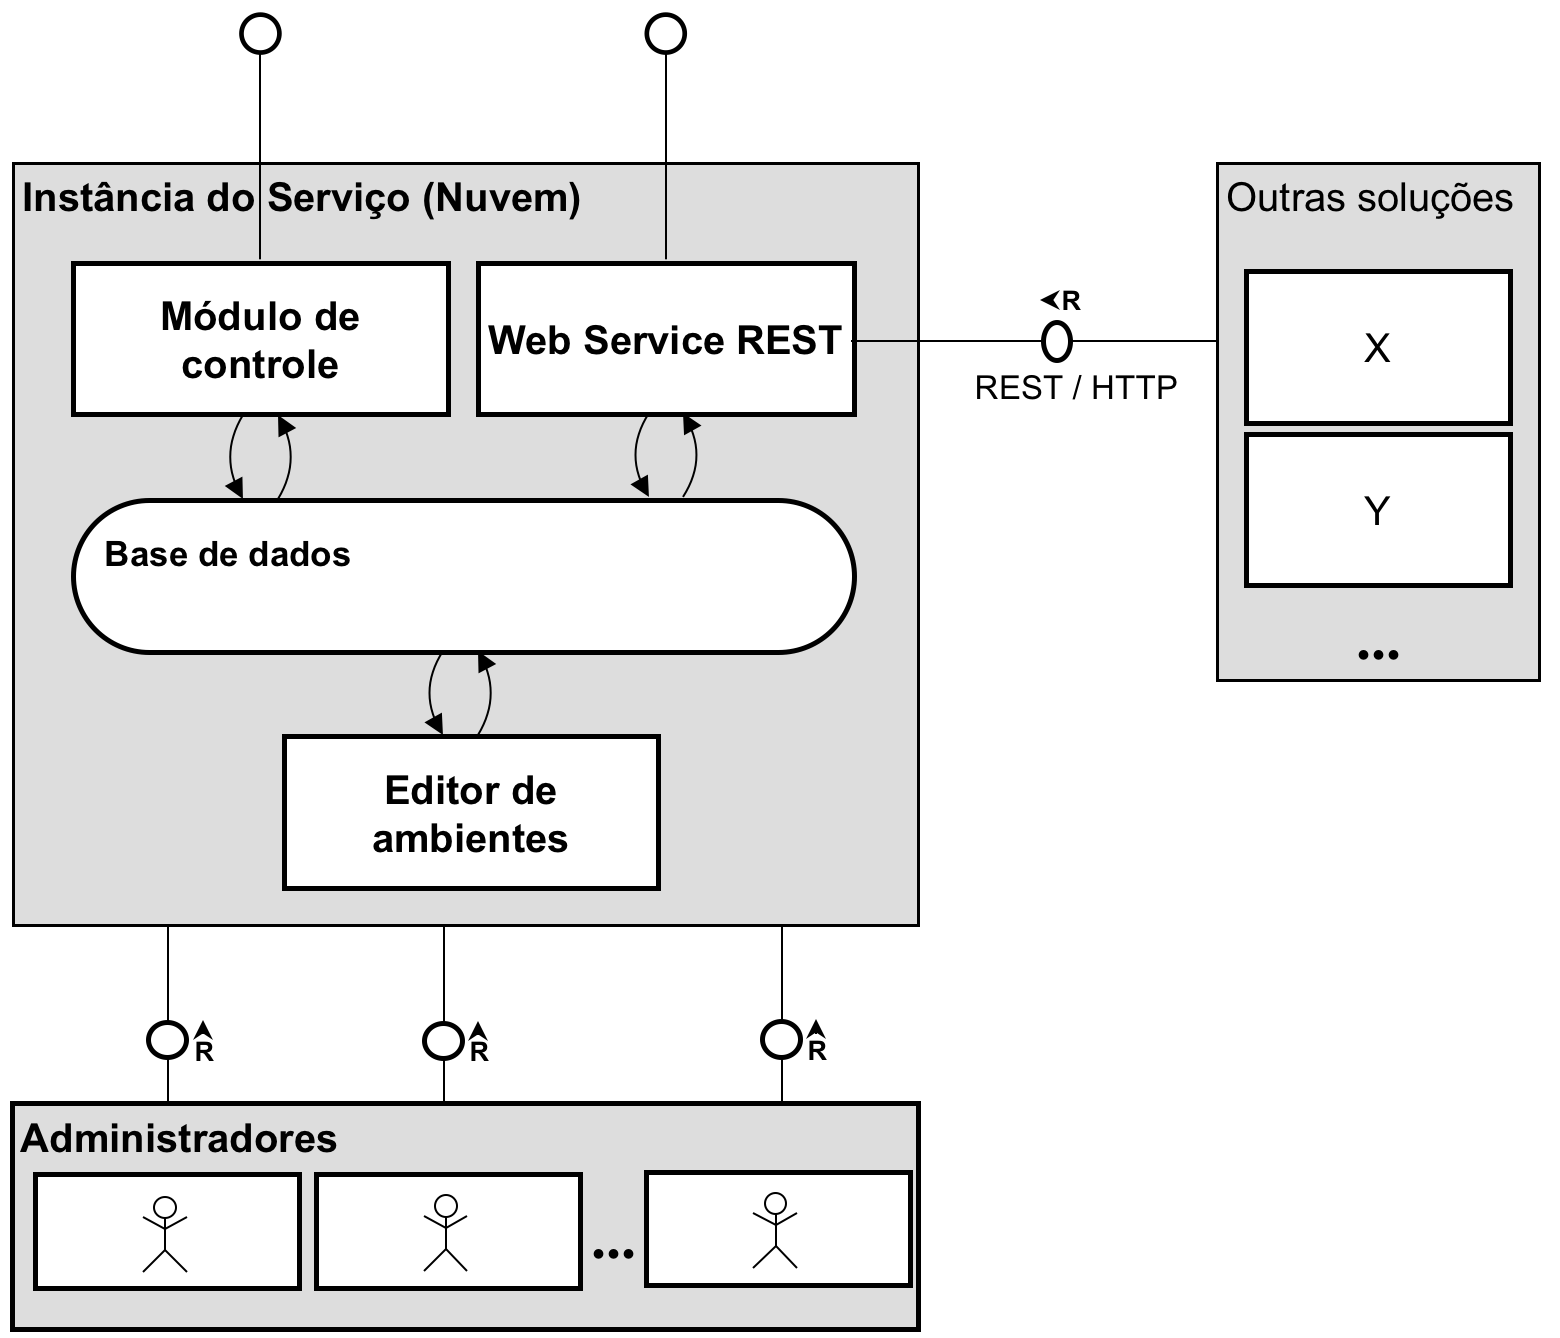
\includegraphics[width=\textwidth]{imgs/arquiteturaServico.png}
		\fonte{Elaborado pelo autor.}
	\end{minipage}
\end{figure}
\FloatBarrier

	\subsubsection{Editor de ambientes}
O editor de ambientes é a ferramenta através da qual os administradores mapeiam o ambiente existente para dentro do modelo. A edição é totalmente visual. Os administradores criam uma representação bidimensional do ambiente, onde devem ser definidos os locais e recursos que podem ser escolhidos como destino pelo usuário, os trechos e caminhos que podem ser percorridos pelos usuários para chegar a algum destino e também indicam os locais onde estão espalhados os beacons.

Para auxiliar durante o mapeamento do ambiente, o modelo permite visualizar áreas não cobertas pelo alcance dos beacons e também oferece sugestões de posicionamento otimizado dos beacons. Os dados são persistidos na base principal do modelo.

	\subsubsection{Módulo de controle}
O módulo de controle mantem informações e referências a todas as instâncias da aplicação servidor em execução. Este componente é o responsável por criar e executar uma nova instância, bem como encerrar sua execução, a fim de que a camada de serviço do Insight mantenha conhecimento de todas as instâncias. Ele controla também informações de histórico a respeito da execução das instâncias e de todas as sincronizações ocorridas, tanto por parte da aplicação cliente como por parte das instâncias, para fins de controle e gerenciamento do Insight. 

Através dele é feito o gerenciamento dos aspectos de segurança e infraestrutura do modelo, como por exemplo a criação de usuários administradores e monitoramento da base de dados.

O modulo de controle oferece um painel onde podem ser monitoradas em tempo real informações relevantes sobre o estado das instâncias, usuários ativos no momento, pedidos de ajuda e outras informações analíticas do modelo. 

	\subsubsection{Base de dados}
A base de dados da camada de serviço é o principal repositório de informações do Insight. Nela ficam armazenados todo o cadastro dos beacons, rotas e locais existentes no modelo. Todas as informações relacionadas aos locais existentes são armazenadas em forma de grafos.

Os dados armazenados são acessados através do web service REST de cada instância. Desta forma, as informações são acessíveis independentemente da plataforma utilizada.

	\subsubsection{Coleção de instâncias}
A coleção de instâncias é o conjunto de todas as cópias da aplicação servidor sendo executadas no momento. 
O ciclo de vida de cada instância é gerenciado pelo módulo de controle.
Mais detalhes sobre aplicação servidor são apresentados na seção \ref{componentesAplicacaoServidor}.

	\subsubsection{Outras soluções}
Um importante aspecto do modelo é sua interoperabilidade. O Insight oferece um serviço completo de localização em ambientes internos. Aliado com a infraestrutura de localização formada pelos beacons dispostos no ambiente, diversas aplicações são possíveis. Cada empresa ou organização que adota o Insight pode fazer uso dos dados do modelo para desenvolver novas soluções de localização em suas dependências, aproveitando toda a infraestrutura já existente para evitar custos. 

Os dados são expostos via web service REST, permitindo que sejam consumidos por qualquer plataforma, oferecendo flexibilidade para as soluções desenvolvidas. 






\subsection{Componentes da aplicação servidor}\label{componentesAplicacaoServidor}
Nesta seção são apresentados cada um dos componentes mostrados na Figura \ref{fig:arquiteturaInstancia}, que formam a arquitetura da aplicação servidor do Insight.

Cada instância roda em servidor físico específico, com seus memória, processamento e armazenamento próprios, garantindo estabilidade e disponibilidade sem prejudicar a performance. Não há limite para quantas instâncias podem ser executadas ao mesmo tempo e cada uma é independente, não possuindo qualquer conhecimento sobre as outras instâncias existentes.

\FloatBarrier
\begin{figure}[!ht]
	\caption{Diagrama de blocos da arquitetura da aplicação servidor}
	\label{fig:arquiteturaInstancia}
	\centering%
	\begin{minipage}{.5\textwidth}
		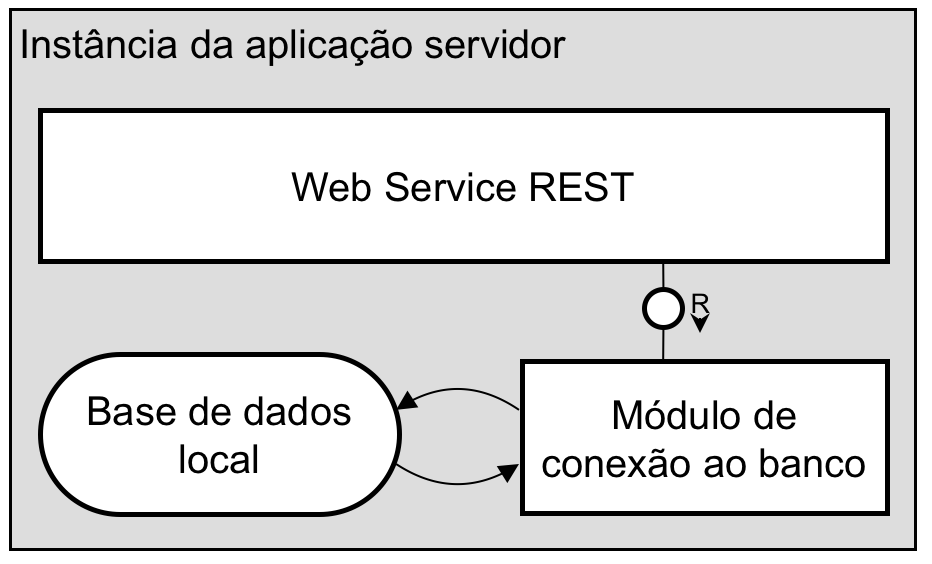
\includegraphics[width=\textwidth]{imgs/arquiteturaInstancia.png}
		\fonte{Elaborado pelo autor.}
	\end{minipage}
\end{figure}
\FloatBarrier

\subsubsection{Web service REST}
O web service REST de cada instância é o responsável por expor aos clientes os dados armazenados na base de dados. Segundo \citetexto{richardson2008restful}, REST é um padrão amplamente utilizado na comunicação entre sistemas, devido a sua capacidade de simplificar o acesso mesmo a dados bastante complexos. O padrão REST não é limitado a alguma plataforma específica, de forma que clientes em quaisquer sistemas sejam facilmente para consumir web services REST. Ainda segundo o autor, uma solução que faz uso do padrão REST é chamada de RESTful.

Através deste componente é realizada a comunicação e a interoperabilidade do Insight. Ele recebe as requisições de dados e então as direciona ao módulo de conexão ao banco de dados, que, por sua vez, determina onde será buscada a informação. As requisições podem originar de outras soluções ou então de clientes Insight sincronizando seus dados.

Este componente também é responsável pela capacidade do Insight de lidar com mudanças dinâmicas no ambiente. Os clientes obtêm as mudanças que ocorreram no ambiente consultando mais frequentemente o web service.

\subsubsection{Módulo de conexão ao banco}
Esse módulo é responsável por realizar todas as operações que necessitam de acesso ao banco de dados, bem como gerenciar todas as conexões da instância com a base de dados. Ele mantem registro das últimas consultas feitas a base de dados bem como dos dados retornados por ela. Desta forma, quando uma nova requisição chega do web service ele pode determinar quem consultar, o cache da instância ou a base de dados principal do modelo. 

\subsubsection{Base de dados local}
A base de dados local serve como um ponto de consulta intermediario entre o web service REST da instância e a base de dados localizada na camada de serviço do Insight. Ela mantem em cache uma cópia temporária das informações que foram buscadas recentemente da base principal. Tal mecanismo tem por fim melhorar o tempo de resposta do modelo às requisições feitas pelos clientes ou por soluções externas que também consomem os dados, uma vez que uma consulta ao cache da instância é mais rápida do que uma consulta até a base de dados localizada na camada de serviço do modelo.

\subsection{Modelo de contexto}
No Insight, a sensibilidade ao contexto do usuário é importante para que o modelo possa ser utilizado da forma mais intuitiva possível. Devido à natureza do modelo, a informação mais relevante é a localização do usuário. Ela será utilizada em três momentos. O primeiro é quando o usuário deseja obter uma rota até algum destino, a localização será utilizada para definir automaticamente o ponto inicial do trajeto como o ponto em que o usuário se encontra. O segundo é durante os deslocamentos, através do contexto o sistema irá automaticamente detectar a evolução do usuário no percurso definido para então fornecer o próximo conjunto de instruções, a fim dispensar qualquer tipo de interação do usuário com o modelo durante o deslocamento. O último também ocorre durante os deslocamentos pelo trajeto, mas é para garantir que usuário seja avisado ao sair do trajeto determinado pelo modelo. Os três momentos oferecerão uma melhor experiência ao usuário.

Para a detecção do contexto serão espalhados beacons Bluetooth pelo ambiente. Estes por sua vez emitirão sinais que serão detectados pelo smartphone do usuário ao entrar na zona de alcance do beacon. O modelo possuirá em seu banco de dados as informações necessárias para obter o posicionamento do beacon ao detectar seu sinal

%=======================================================================
% Metodologia
%=======================================================================
\chapter{Metodologia}
\epigrafecap{The future is already here. It's just not very evenly distributed.}{William Gibson}

Enquadrando o presente trabalho na classificação apresentada em \citetexto{Gerhardt2009}, quanto à natureza da pesquisa, ele se caracteriza como uma pesquisa aplicada, pois objetiva gerar conhecimentos para aplicação prática dirigidos à solução de um problema específico que é a navegação e localização de deficientes visuais. A abordagem do trabalho é qualitativa e, do ponto de vista dos objetivos, é uma pesquisa exploratória e descritiva, buscando resultar em um modelo acessível de localização e navegação em ambientes internos. O procedimento técnico utilizado para a construção da pesquisa é a pesquisa bibliográfica.

	\section{Aspectos de implementação}
Nesta seção são comentados pontos relacionados ao desenvolvimento do protótipo e técnicos do modelo, como por exemplo casos de uso, requisitos funcionais e não funcionais, ferramentas e tecnologias utilizadas.

	\subsection{Requisitos e casos de uso}  
O diagrama de casos de uso apresentado na Figura \ref{fig:diagramaCasosDeUso} foi desenvolvido para auxiliar na fase de elicitação de requisitos, fornecer uma melhor visualização das funcionalidades da solução e também mostrar quais são os atores envolvidos com cada uma delas. O diagrama foi construído levando em consideração as características encontradas nos trabalhos relacionados, bem como as informações presentes no referencial teórico deste trabalho.


\begin{figure}[!ht]
	\caption{Diagrama de casos de uso do Insight}
	\label{fig:diagramaCasosDeUso}
	\centering%
	\begin{minipage}{,9\textwidth}
		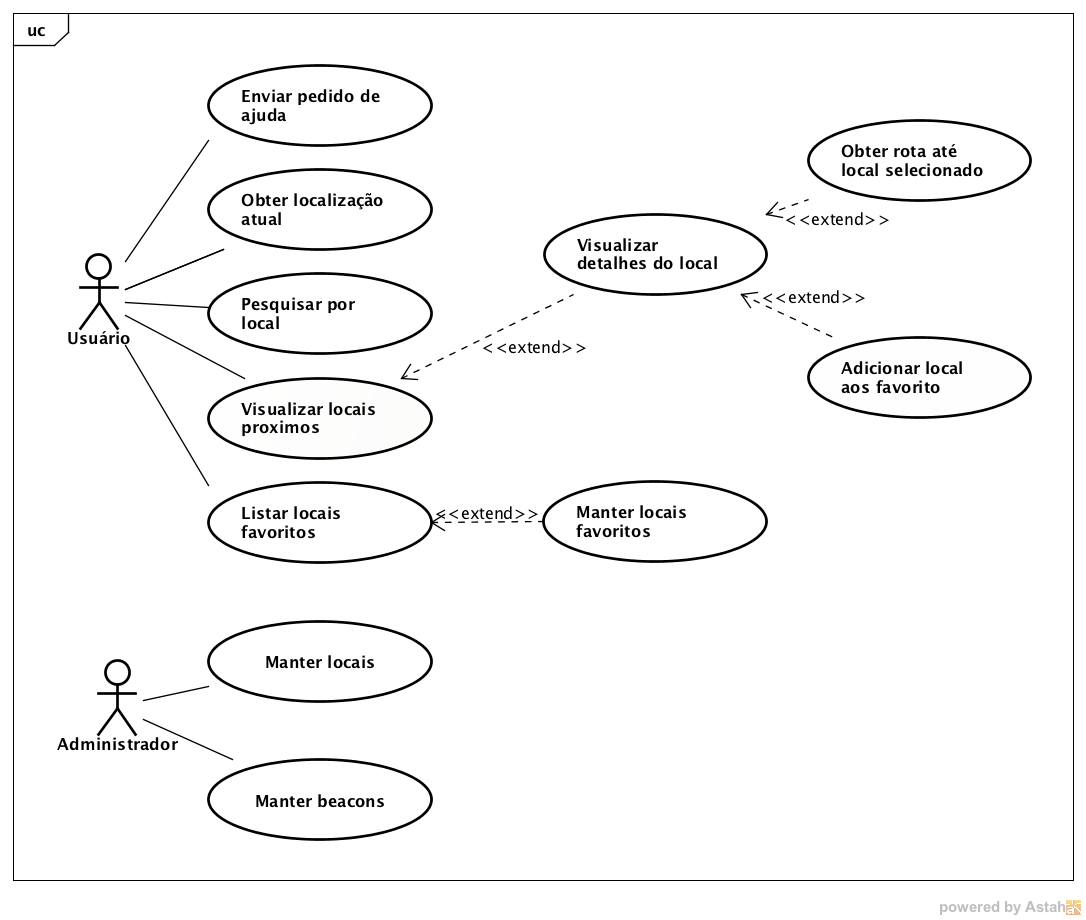
\includegraphics[width=\textwidth]{imgs/casosDeUso}
		\fonte{Elaborado pelo autor.}
	\end{minipage}
\end{figure}
	

A listagem dos requisitos é apresentada nas seções subsequentes, sendo dividida entre requisitos funcionais e requisitos não funcionais.

\subsection{Requisitos funcionais} 
Nesta seção são apresentados os requisitos funcionais elicitados para o modelo Insight. Cada requisito funcional corresponde a uma funcionalidade presente na solução, a fim de que usuários possam desempenhar suas ações. Para a definição dos requisitos foi levado em consideração que o sistema possui dois tipos de usuários: usuários comuns e administradores.

Os requisitos funcionais elicitados para o modelo são:

\begin{itemize}
	% USER
	\item \textbf{RF01 - Obter localização atual:} o usuário poderá obter sua localização atual a qualquer momento.
		
	\item \textbf{RF02 - Visualizar locais próximos:} o usuário poderá visualizar os locais próximos a si, ordenados pela distância até o local.
		
	\item \textbf{RF03 - Pesquisar por local:} o usuário poderá pesquisar entre os locais disponíveis usando critérios como nome ou categoria.
		
	\item \textbf{RF04 - Visualizar detalhes do local:} o usuário poderá visualizar informações específicas do local selecionado, tais como nome, descrição, categoria e distância até ele.

	\item \textbf{RF05 - Obter rota até local selecionado:} o usuário poderá obter uma rota até o local selecionado, partindo do seu local atual.

	\item \textbf{RF06 - Listar locais favoritos:} o usuário poderá visualizar uma lista com os locais marcados como seus favoritos.
		
	\item \textbf{RF07 - Manter locais favoritos:} o usuário poderá adicionar ou excluir locais da lista de locais favoritos.
		
	\item \textbf{RF08 - Mensagem de boas-vindas:} o sistema deverá detectar quando o usuário chega no ambiente e enviar uma notificação ao usuário perguntando se ele deseja usar o cliente.

	\item \textbf{RF09 - Enviar pedido de ajuda:} o usuário poderá enviar aos administradores um pedido de ajuda informando o seu último local conhecido, para que alguém seja enviado para socorrer o usuário.
		
	% ADMIN
	\item \textbf{RF10 - Manter locais:} o administrador poderá adicionar, editar, ou excluir locais e rotas cadastrados no modelo.
		
	\item \textbf{RF11 - Manter beacons:} o administrador poderá adicionar, editar, ou excluir beacons cadastrados no modelo.

	\item \textbf{RF12 - Sincronização:} o administrator poderá alterar a periodicidade das sincronizações do cliente com o servidor.

\end{itemize}

\subsection{Requisitos não funcionais}
Nesta seção são apresentados os requisitos não funcionais elicitados para o modelo Insight. Os requisitos não funcionais descrevem aspectos internos da aplicação no que diz respeito ao desempenho, confiabilidade, interoperabilidade, mobilidade, disponibilidade, segurança e usabilidade.

Os requisitos não funcionais elicitados para o modelo Insight são:

\begin{itemize}
	\item \textbf{RNF01 - Escalabilidade e disponibilidade - Serviço na nuvem:} A aplicação servidor será uma aplicação web.

	\item \textbf{RNF02 - Interoperabilidade - Serviços web REST:} a aplicação servidor disponibilizará web services utilizando o padrão Representational State Transfer (REST) para realizar a integração com os clientes e outras soluções.

	\item \textbf{RNF03 - Interoperabilidade - JSON:} o sistema usará o padrão Javascript Object Notation (JSON) para a transferência de informações a partir do servidor REST, a fim de facilitar a comunicação com os clientes e outras soluções.

	\item \textbf{RNF04 - Portabilidade - Clientes para dispositivos móveis:} a aplicação cliente será utilizado em smartphones ou tablets.

	\item \textbf{RNF05 - Usabilidade - Base de dados local:} O cliente deverá conter uma cópia local do banco de dados localizado na nuvem.

	\item \textbf{RNF06 - Confiabilidade - Sincronização:} O cliente deverá periodicamente sincronizar sua base de dados com a base de dados na nuvem.

	\item \textbf{RNF07 - Usabilidade - Adaptação ao contexto:} o cliente deverá identificar o contexto do usuário através do uso da localização, a fim de exibir os locais mais relevantes e fornecer os próximos passos da navegação.

	\item \textbf{RNF08 - Usabilidade - Comandos por gestos:} o cliente deverá permitir a interação do usuário através de gestos.

	\item \textbf{RNF09 - Usabilidade - Comandos por voz:} o cliente deverá permitir a interação do usuário através de comandos de voz.

	\item \textbf{RNF10 - Acessibilidade - Feedback por voz:} o cliente deverá fornecer informações ao usuário através do uso de voz.

	\item \textbf{RNF11 - Acessibilidade - Feedback tátil:} o cliente deverá fornecer informações ao usuário através do uso de alertas vibratórios.

	\item \textbf{RNF12 - Acessibilidade - Discrição:} o modelo deve poder ser utilizado a partir de hardware leve e discreto.

	\item \textbf{RNF13 - Usabilidade - Interferência:} o modelo não deve interferir em outras ferramentas que o usuário possa estar usando para se deslocar.

	\item \textbf{RNF14 - Confiabilidade - Cache:} cada instância deverá manter uma cópia local temporaria dos dados que forem obtidos da base principal, afim de otimizar o tempo de resposta.

	\item \textbf{RNF15 - Confiabilidade - Cache:} a instância deverá, a cada consulta ao banco de dados, verificar se os dados já existem na base local, antes de consultar na base principal.

	\item \textbf{RNF16 - Desempenho - Formato de armazenamento:} o modelo deve armazenar as informações relativas a rotas no formato de grafos.

	\item \textbf{RNF17 - Desempenho - Calculo de rotas:} as rotas deverão ser calculadas através do algoritmo de Dijkstra.

\end{itemize}

A partir dos requisitos funcionais e não funcionais, é possível perceber que os dispositivos móveis são a ferramenta ideal para uso do modelo.

\subsection{Passos metodológicos}

O trabalho de modelagem e desenvolvimento do Insight foi divido em 9 passos metodológicos apresentados na Figura \ref{fig:passosMetodologicos}. Os passos 1 a 6 foram realizados no presente trabalho. Os demais passos serão realizados na disciplina Trabalho de Conclusão II, que também compreende os requisitos para a colação de grau da Universidade do Vale do Rio dos Sinos (UNISINOS).

\begin{figure}[!ht]
	\caption{Passos metodológicos}
	\label{fig:passosMetodologicos}
	\centering%
	\begin{minipage}{.7\textwidth}
		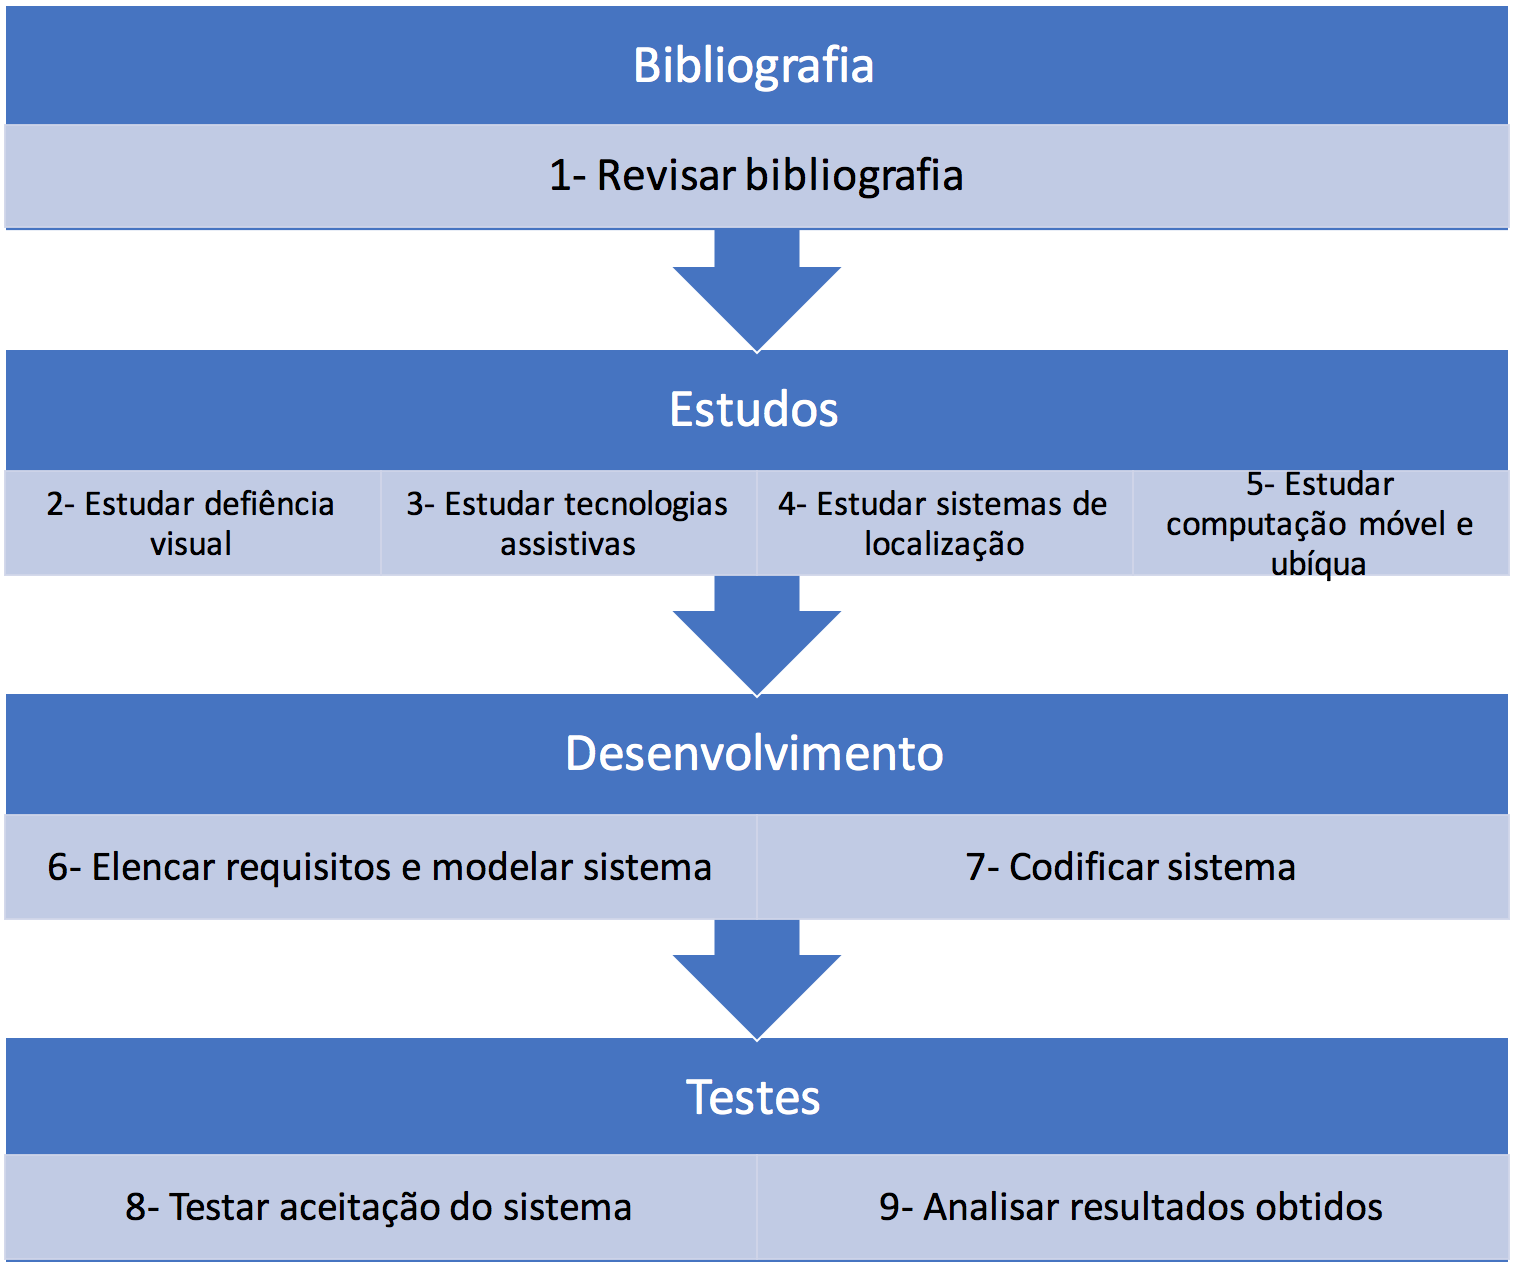
\includegraphics[width=\textwidth]{imgs/passosMetodologicos}
		\fonte{Elaborado pelo autor.}
	\end{minipage}
\end{figure}

A seguir são apresentados brevemente cada um dos passos concebidos:

% passos
\begin{enumerate}
	%	1
	\item \textbf{Revisar bibliografia:} Pesquisa bibliográfica objetivando descobrir trabalhos envolvendo o tema em questão. Realizar leitura e resumo dos trabalhos relevantes encontrados, e, com isso, criar uma fundamentação teórica adequada para o desenvolvimento desta pesquisa.
	%	2
    \item \textbf{Realizar estudo sobre deficiência visual:} Estudar essa deficiência em busca de compreender a maneira com que ela afeta seus portadores, e também o processo mental realizado por eles durante seu deslocamento, tanto em ambientes familiares como desconhecidos, a fim de criar uma abstração desse processo aplicando-a ao modelo.
	%	3
    \item \textbf{Realizar estudo sobre tecnologias assistivas:} Estudar e verificar quais tecnologias já foram aplicadas na acessibilidade, avaliando quais podem ser utilizadas no desenvolvimento do modelo para melhor atender às necessidades dos PDV.
	%	4
    \item \textbf{Realizar estudo sobre sistemas de localização:} Estudo buscando compreender o estado da arte dos sistemas de localização, identificando características que devem ser aplicadas em um sistema acessível destinado a PDV.
	%	5
    \item \textbf{Realizar estudo sobre computação móvel e ubíqua:} Estudar o conceito de computação ubíqua, bem como conceitos relacionados, em busca de ideias que podem ser aplicadas no desenvolvimento e no uso do presente modelo, tornando-o mais natural e transparente possível aos usuários.
    %	6
    \item \textbf{Elencar requisitos e modelar o sistema:} Elaborar os modelos necessários para o posterior desenvolvimento do sistema, utilizando a linguagem UML.
    %	7
    \item \textbf{Codificar sistema:} Codificar o sistema de acordo com a modelagem realizada.
	%	8
	\item \textbf{Testar aceitação do sistema:} Codificar uma prévia do modelo desenvolvido de modo que ela possa ser avaliada em campo.
	%	9
	\item \textbf{Analisar resultados dos testes:} Realizar análise dos resultados obtidos através dos questionários, traçando uma conclusão do trabalho desenvolvido. Posteriormente, verificando os benefícios e dificuldades apresentados pelo sistema aos participantes, a fim de estabelecer ajustes e correções, bem como trabalhos futuros.
\end{enumerate}

	\section{Metodologia de avaliação}
A avaliação do modelo proposto se dará após a implementação de um protótipo, tendo duas formas previstas de avaliação. A primeira consiste na avaliação por cenários e a segunda na avaliação por usabilidade. Ambas possibilitarão detectar problemas pontuais e verificar a adaptação ao usuário ao sistema durante o período de uso. O resultado das análises permitirá identificar a eficácia do sistema e possibilitará elencar melhorias e/ou trabalhos futuros relacionados ao tema.

O protótipo será desenvolvido para a plataforma Android, usando recursos nativos do sistema operacional disponibilizadas através da linguagem Java e o ambiente de desenvolvimento Android Studio.

\subsection{Avaliação por cenários}
A comunidade cientifica tem utilizado cenários para avaliação de sistemas sensíveis ao contexto, conforme \citetexto{Satyanarayanan2001} e \citetexto{dey2001understanding}. Seguindo essa abordagem, serão criados dois cenários para teste do Insight. Ambos são baseados nos cenários descritos por \citetexto{Falk2013}, serão conduzidos por um usuário se deslocando pelo ambiente portando um smartphone com um protótipo do modelo Insight. 

Recursos e locais fictícios serão mapeados no modelo, afim de simular recursos existentes no campus da Universidade do Vale do Rio dos Sinos\footnote{Site da Unisinos http://www.unisinos.br/} (Unisinos).
O cenário 1 simulará a chegada de um aluno com deficiência visual à universidade e sua interação inicial com os recursos fornecidos pelo modelo. O cenário 2 demonstrará a interação do usuário com os recursos espalhados pelo ambiente da Universidade, explorando funcionalidades adicionais.

\subsection{Avaliação por usabilidade}
Na expectativa de adquirir beacons BLE também é previsto uma avaliação com foco na usabilidade do protótipo. Usabilidade é definida na ISO 9244-11 como "a medida em que um produto pode ser usado pelos seus usuários para atingir objetivos com efetividade, eficiência e satisfação em um determinado contexto de uso (usuários, tarefas, equipamentos e ambientes)". \cite{ISO9241}.
Nesta forma de avaliação, PDV que tenham interesse em colaborar com a pesquisa serão convidados a participar. Após o experimento, os usuários serão responderão um questionário, preparado seguindo a metodologia Technology Acceptance Model (TAM). No questionário os usuários irão utilizar a escala de Likert, proposta por \citetexto{likert1932technique}, para opinar sobre o protótipo e o modelo propostos. O TAM, proposto por \citetexto{davis1989perceived} e posteriormente aprimorado por \citetexto{yoon2007convenience}, define dois critérios para o aceite de uma tecnologia. O primeiro mede a percepção do usuário sobre a utilidade da tecnologia em avaliação, e o segundo mede a facilidade de uso, através da usabilidade e características do sistema. O primeiro critério define se a tecnologia é capaz de auxiliar o usuário na execução de suas tarefas, enquanto o segundo determina se ela pode ser usada com o mínimo de esforço. A escala de Likert define 5 alternativas para cada afirmação, sendo elas "Concordo completamente", "Concordo", "Indiferente", "Discordo", "Discordo completamente".

\chapter{Conclusão}
\epigrafecap{For millions of years, mankind lived just like the animals. Then something happened which unleashed the power of our imagination. We learned to talk and we learned to listen...}{Stephen Hawking}

O presente trabalho propôs um modelo de arquitetura para um serviço de localização acessível. Para isso, foram realizados estudos de trabalhos relacionados com o mesmo objetivo e também pesquisas sobre sistemas de localização, sensibilidade ao contexto, tecnologias aplicadas em localização e deficiência visual. Através dele é possível compreender os principais conceitos da área computação ubíqua, da acessibilidade no Brasil e na internet, das tecnologias assistivas e também entender um pouco sobre deficiência visual.

Inicialmente uma grande pesquisa bibliográfica foi realizada afim de conhecer o estado da arte na área da acessibilidade. Os trabalhos mais relevantes encontrados foram listados na seção \ref{cap:trabalhosRelacionados}. O estudo dos trabalhos relacionados possibilitou a criação de um modelo focado no usuário que leva em consideração a usabilidade do sistema. Denominado Insight, ele atua auxiliando usuários PDV em seu deslocamento em ambientes internos. 

Para a criação do modelo, foram utilizadas as seguintes etapas do desenvolvimento de um software: análise do problema, criação dos casos de uso, especificação dos requisitos e modelagem da arquitetura da solução proposta. Todas essas fases foram muito importantes por permitir colocar em prática alguns dos conceitos aprendidos durante o curso de graduação.

Esta dissertação é requisito parcial para obtenção do título de Bacharel em Ciência da Computação pela Universidade do Vale do Rio dos Sinos. Assim sendo, as demais etapas estabelecidas neste modelo, como o desenvolvimento, testes e validação de um protótipo, serão realizas em um trabalho complementar que descreverá estas fases baseado no modelo aqui apresentado.

\section{Comparação entre os trabalhos estudados e o modelo proposto}
Para finalizar o presente trabalho, é apresentado um comparativo entre o modelo proposto e os trabalhos apresentados no Capitulo \ref{cap:trabalhosRelacionados}. Para tal, foram adicionados as informações do modelo proposto à Tabela \ref{tab:trabalalhosRelacionados}, obtendo como resultado a Tabela \ref{tab:trabalalhosRelacionadosEInsight}.

Analisando a tabela, é fácil perceber que todos os trabalhos são semelhantes em questão do acesso através de dispositivos móveis, da comunicação através da internet e da exigência de hardware específico. Apenas o PERCEPT se destaca negativamente exigindo hardware customizado para utilização do modelo.

O Insight se destaca dos trabalhos relacionados em diversos pontos:
\begin{itemize}
	\item Na utilização da tecnologia Bluetooth Low Energy combinada com a área de abrangência em ambientes internos, enquanto o outro trabalho que utiliza a mesma tecnologia possui alcance limitado ao entorno de zonas em obras.

	\item Nas formas de interação do usuário com o modelo. O Insight é o único que suporta a combinação toques, gestos e voz. Os trabalhos relacionados suportam apenas toques ou então toques e gestos.

	\item Juntamente com o Tirésias, o modelo tem suporte a interoperabilidade com outras soluções. Porém, o Insight usa web services REST enquanto o Tirésias faz uso de agentes.

	\item O Insight é o único modelo que usa uma biblioteca dedicada à construção de soluções de localização, fornecendo uma base pronta o desenvolvimento de modelos para localização em ambientes internos com beacons BLE.

	\item A arquitetura do Insight é caracterizada como serviço distribuído na nuvem. Isso garante a infraestrutura para uma solução escalável e altamente disponível aos usuários. Todos os trabalhos relacionados fazem uso da estrutura cliente-servidor, menos escalável que o Insight.

	\item O Insight aplica a ciência de contexto para se adaptar as necessidades do usuário. Dos quatro trabalhos relacionados, apenas 2 também usam o contexto para reagir às mudanças no ambiente do usuário.
\end{itemize}

Informações como linguagem de programação, banco de dados e sistema operacional não podem ser comparados visto que essas definições ocorrerão posteriormente, na fase de desenvolvimento do protótipo Insight.

\FloatBarrier
\begin{table}
	\caption{Tabela comparativa entre os trabalhos relacionados e o Insight}
	\label{tab:trabalalhosRelacionadosEInsight}
	\centering%
	\begin{minipage}{1\textwidth}
	\begin{adjustbox}{max width=\textwidth}
		\begin{tabular}{ | p{3cm} | p{3cm} | p{3cm} | p{3cm} | p{3cm} | p{3cm} | }
\hline
	 & Percept & UCAT & Navigation System for Workzone & Tirésias & Insight \\ \hline
	Método de localização & RFID & Bluetooth 2.1 & Bluetooth LE & GPS & Bluetooth LE \\ \hline
	Abrangência & Indoor & Indoor e outdoor & Zonas em obras & Indoor & Indoor \\ \hline
	Ambientes dinâmicos & Não especificado & Não especificado & Não especificado & Não especificado & Sim \\ \hline
	Meio de acesso & Dispositivos móveis & Dispositivos móveis & Dispositivos móveis & Dispositivos móveis & Dispositivos móveis \\ \hline
	Interface do utilizador & Toques & Toques e gestos & Toques & Toques e gestos & Toques, gestos e voz \\ \hline
	Hardware específico & Sim & Não & Não & Não & Não \\ \hline
	Comunicação & Internet ou intranet & Internet & Internet & Internet ou intranet & Internet ou intranet \\ \hline
	Interoperabilidade & Não & Não & Não & Sim, através de agentes & Sim, através de web services REST \\ \hline
	Adaptação & Não & Sim, através de sensibilidade ao contexto & Não & Sim, através de sensibilidade ao contexto & Sim, através de sensibilidade ao contexto \\ \hline
	Banco de dados & Postgres & SQLite & MySQL & Não especificado & Não especificado \\ \hline
	Linguagem & Java & Java & Java & Objective-C & Não especificado \\ \hline
	Sistema operacional & Android & Android & Android & iOS & Não especificado \\ \hline
	Bibliotecas utilizadas & Não especificado & Não especificado & Não especificado & Não especificado & Indoo.rs \\ \hline
	Hardware & Luva equipada c/ leitor RFID e dispositivo móvel c/ Bluetooth & Dispositivos móveis c/ Bluetooth & Dispositivos móveis c/ Bluetooth & Dispositivos Móveis c/ GPS & Dispostivos móveis com Bluetooth \\ \hline
	Arquitetura & Cliente-servidor & Cliente-servidor & Cliente-servidor & Cliente-servidor & Distribuída (nuvem) \\ \hline
		\end{tabular}
		\end{adjustbox}
		\fonte{Elaborado pelo autor.}
	\end{minipage}
\end{table}
\FloatBarrier
	
	\section{Trabalhos futuros}
Alguns aspectos da modelagem das informações foram simplificados durante a construção do modelo, devido à natureza volátil dos requisitos necessários para propriamente os modelar. Todavia, o presente trabalho pode ser continuado e a sua evolução pode considerar mais informações sobre os trajetos e a dificuldade que eles oferecem. Outro ponto seria indicar aos usuários os locais que oferecem serviços especializado a deficientes visuais.

Algumas sugestões para o desenvolvimento futuro deste modelo são:

\begin{itemize}
	\item Tendo em vista que um dos objetivos deste trabalho é facilitar o acesso dos PDV a oportunidades advindas da educação, adicionar a possibilidade de integração com os sistemas acadêmicos das Universidades. Dessa forma, alunos poderiam utilizar o modelo e, baseado no contexto, automaticamente obter direções para os locais onde tem aula quando chegam ao campus.

	\item Considerar a dificuldade do percurso no cálculo das rotas que são apresentadas ao usuário, excluindo caminhos que tenham escadas ou aclives e decliveis acentuados, fornecendo o caminho mais fácil ao usuário e contribuindo para a segurança dos PDV.

	\item Inclusão de um novo meio de acesso ao sistema através de dispositivos vestíveis. Estes permitem que os usuários possam trafegar com as mãos livres para outras atividades.
\end{itemize}

%=======================================================================
% Referências
%=======================================================================
\bibliography{bibliografia}

\end{document}